% !TEX root = ../sethomas_thesis_main.tex

\chapter{Predicting the Shape Memory Effect}\label{chap:sma-model}
\section{Introduction}
% Intro to thermal SMAs (mention magnetic)
% Type of TSMA (NiTi, CuAl)
    % Mechanical prop of NiTi (table)
% SME and SE
% SME graph A to M, detw to tw
% Phase transformations
\begin{figure}[hbt]
    \centering
    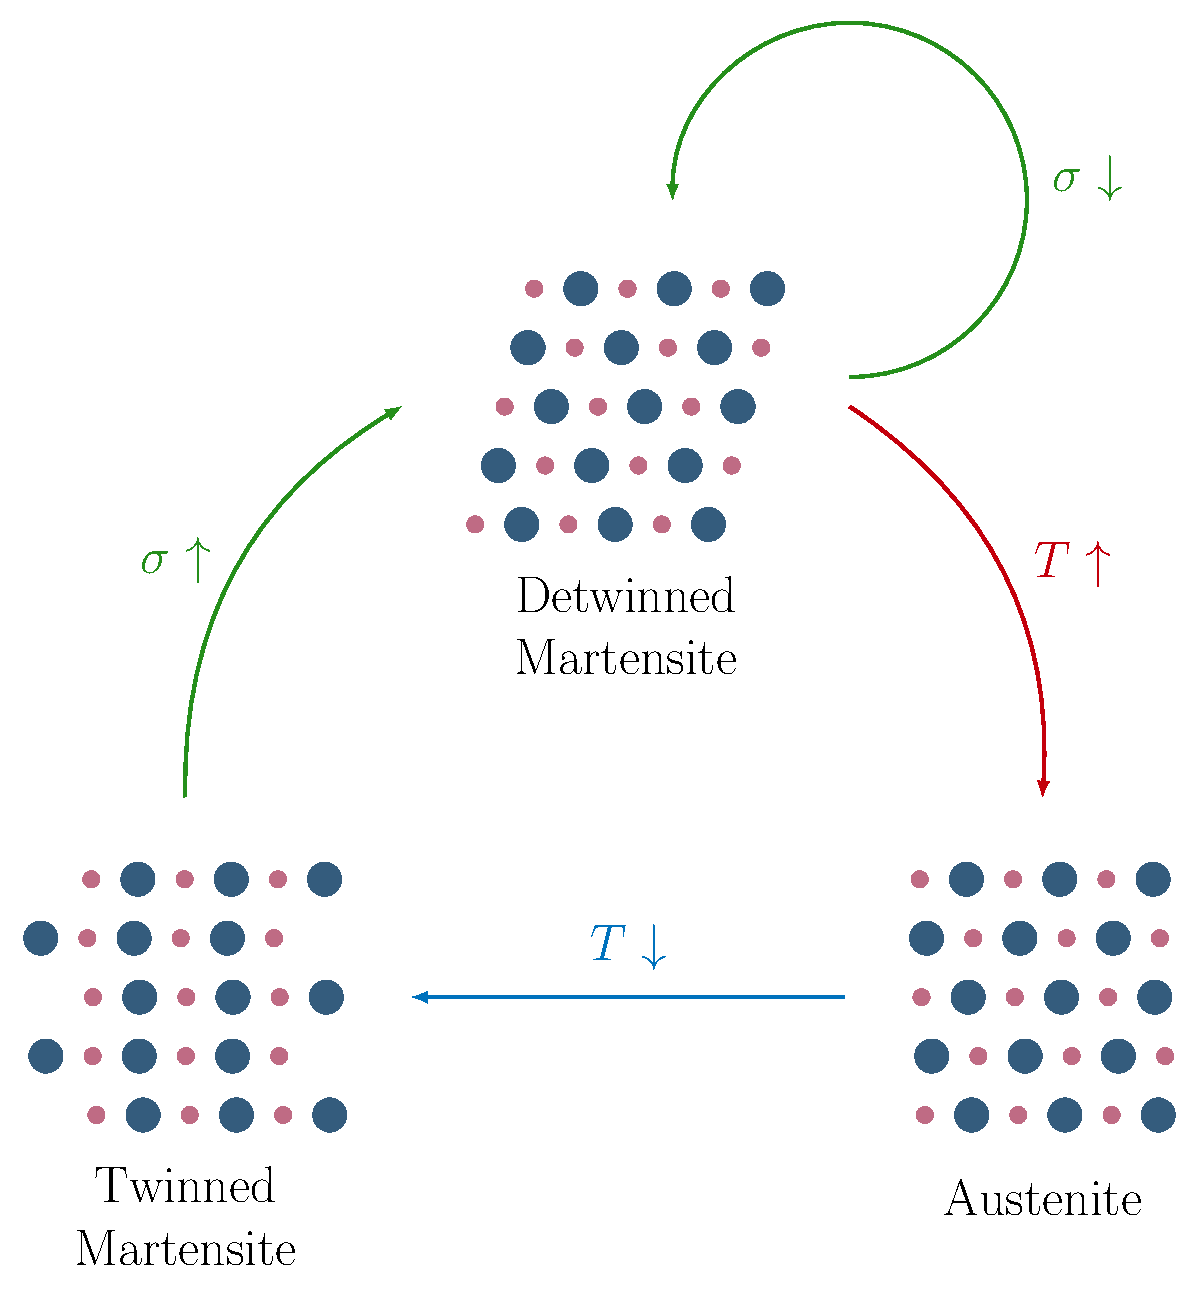
\includegraphics[width=0.6\textwidth]{images/chap2/sma-phases.pdf}
    \caption{A schematic representation of the Shape Memory Effect (SME) showing the different phase transformations and crystal structures.}
    \label{fig:sma-phases}
\end{figure}

\begin{figure}[hbt]
    \centering
    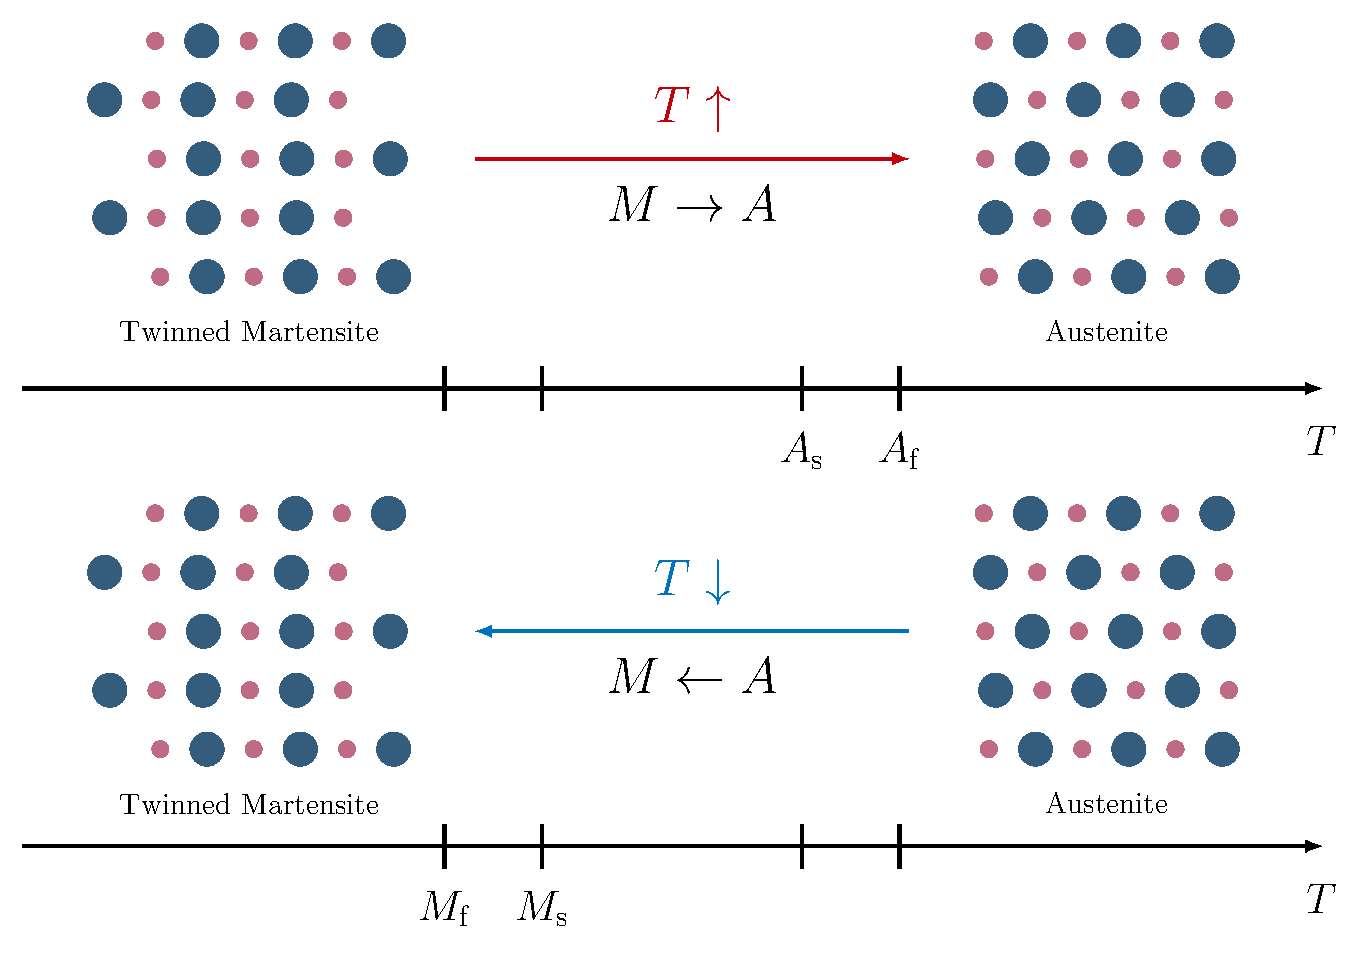
\includegraphics[width=0.75\textwidth]{images/chap2/sma-phase-transformations.pdf}
    \caption{A visual representation of the phase transformations that occur during Shape Memory Effect (SME) under no load.}
    \label{fig:sma-phase-transformations}
\end{figure}

\begin{figure}[hbt]
    \centering
    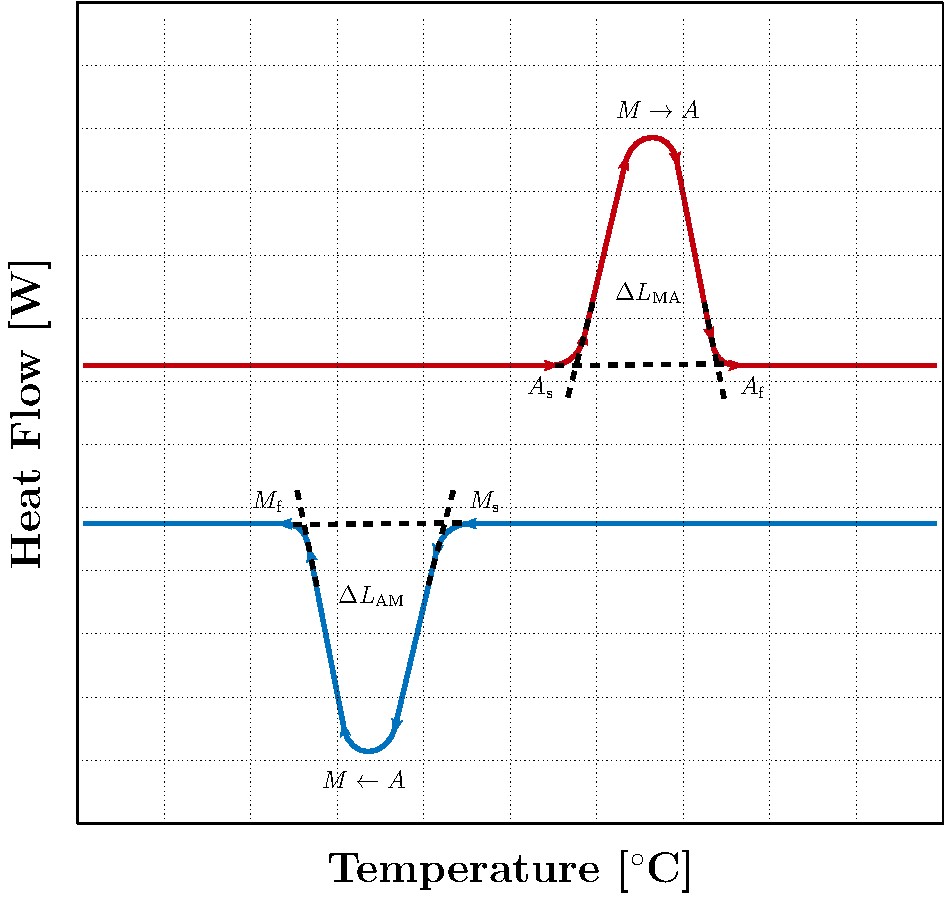
\includegraphics[width=0.75\textwidth]{images/chap2/dsc-graph.pdf}
    \caption{Schematic representation of a differential scanning calorimetry (DSC) graph showing the energy required during the SME.}
    \label{fig:dsc-graph}
\end{figure}

\begin{figure}[hbt]
    \centering
    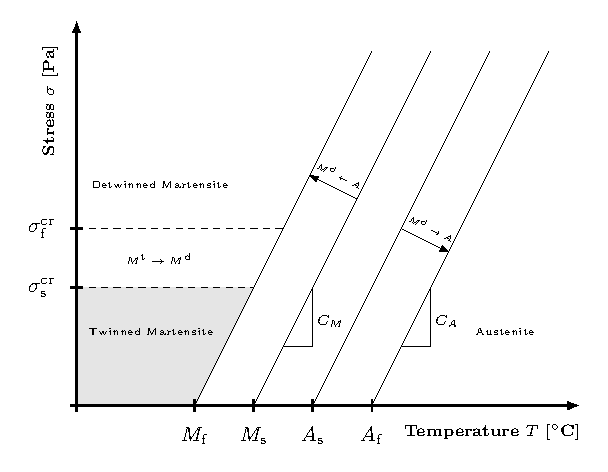
\includegraphics[width=0.75\textwidth]{images/chap2/phase-diagram-graph.pdf}
    \caption{Graphical representation of the phase transformations showing the thermal and mechanical properties of the material. This graph presents the change in the transformation temperature based on the imposed stress on the SMA.}
    \label{fig:phase-diagram-graph}
\end{figure}

\section{Analytical Modelling of the SME}
% Phenomenological modelling
% DSC
% Types and history of models
% Brinson model

As mentioned previously, the shape memory effect is a different process to model analytical due to the different phase transformations and variables. The work by \cite{liangDesignShapeMemory1997} presented a unified one-dimensional phenomenological model that takes into account the M phase transformation. However this model does not accurately describe the detwinning process. The Brinson model in the worky by \cite{brinsonOneDimensionalConstitutiveBehavior1993} improves the model by separating the internal variable into two based on the stress and temperature.

The basic constitutive model presented by Brinson is as follows,
\begin{equation}
  \label{eq:brinson_model_1}
  d\sigma = \frac{\delta\sigma}{\delta\epsilon}d\epsilon + \frac{\delta\sigma}{\delta\xi_S}d\xi_S + \frac{\delta\sigma}{\delta\xi_T}d\xi_T + \frac{\delta\sigma}{\delta T}dT
\end{equation}
 which can be further simplified using constant material functions as
\begin{equation}
  \label{eq:brinson_model_2}
  d\sigma = Dd\epsilon + \Omega_Sd\xi_S + \Omega_Td\xi_T + \Theta dT
\end{equation}
where $D(\epsilon,\xi,T)$ represents the Young's modulus of the SMA material, $\Omega(\epsilon,\xi,T)$ represents the transformation tensor and $\Theta(\epsilon,\xi,T)$ is the thermal coefficient of expansion of the SMA.

An important aspect of the work presented by Brinson was the adaptation of the transformation equations and transformation stresses. The work was able to deduce an analytical model for the detwinning process by adapted the transformations equations present earlier by Liang. For $T > M_\mathrm{s}$ and $\sigma_\mathrm{s}^\mathrm{cr} + C_M(T - M_\mathrm{s}) < \sigma < \sigma_\mathrm{f}^\mathrm{cr} + C_M(T-M_\mathrm{s})$ :

\begin{equation}
  \label{eq:brinson_conv_xis}
  \xi_S = \cos\left(\frac{\pi}{\sigma_\mathrm{s}^\mathrm{cr}-\sigma_\mathrm{f}^\mathrm{cr}}[\sigma - \sigma_\mathrm{f}^\mathrm{cr} - C_M(T-M_\mathrm{s})]\right)\frac{1-\xi_{S0}}{2} + \frac{1+\xi_{S0}}{2}
\end{equation}

\begin{equation}
  \label{eq:brinson_conv_xit}
  \xi_T = \xi_{T0} - \frac{\xi_{T0}}{1-\xi_{S0}}(\xi_S-\xi_{S0})
\end{equation}

Due to the complexity of the shape memory effect, the constitutive model must be divided into three phases : the detwinning process, the stress relaxation and the austenitic transformation. The detwinning process can be calculated by using equation \ref{eq:brinson_conv_xis} combined with equation \ref{eq:brinson_model_2}. The stress relaxation phase occurs when $\xi_S$ is kept constant at 1 and the stress is reduced back to 0. Lastly, the austenitic phase transformation can be calculated using equation \ref{eq:brinson_model_2} and the following equation :

\begin{equation}
  \label{eq:A_transf}
  \xi = \frac{\xi_0}{2}\left\{\cos\left[a_A(T-A_\mathrm{s}-\frac{\sigma}{C_A})\right]+1\right\}
\end{equation}
\begin{equation}
    \label{eq:a-transf_1}
    \xi_S = \xi_{S0} - \frac{\xi_{S0}}{\xi_0}(\xi_0-\xi)
\end{equation}
\begin{equation}
    \label{eq:a-transf_2}
    \xi_T = \xi_{T0} - \frac{\xi_{T0}}{\xi_0}(\xi_0-\xi)
\end{equation}

where $\Ms$ and $\As$ are the Martensitic and Austenitic transformation start temperatures and finish temperatures. While $C_M$ and $C_A$ are material properties that tie the internal stresses to a change in transformation temperatures. More information on the constitutive models and the material constants can be found in work by \cite{brinsonOneDimensionalConstitutiveBehavior1993}. In \cref{fig:brinson-model-stress-strain}, the results of the analytical model based on the Brinson constitutive equations can be observed.

% Temp vs Martensite %
\begin{figure}[hbt]
    \centering
    \resizebox{0.75\textwidth}{!}{%% Creator: Matplotlib, PGF backend
%%
%% To include the figure in your LaTeX document, write
%%   \input{<filename>.pgf}
%%
%% Make sure the required packages are loaded in your preamble
%%   \usepackage{pgf}
%%
%% and, on pdftex
%%   \usepackage[utf8]{inputenc}\DeclareUnicodeCharacter{2212}{-}
%%
%% or, on luatex and xetex
%%   \usepackage{unicode-math}
%%
%% Figures using additional raster images can only be included by \input if
%% they are in the same directory as the main LaTeX file. For loading figures
%% from other directories you can use the `import` package
%%   \usepackage{import}
%%
%% and then include the figures with
%%   \import{<path to file>}{<filename>.pgf}
%%
%% Matplotlib used the following preamble
%%
\begingroup%
\makeatletter%
\begin{pgfpicture}%
\pgfpathrectangle{\pgfpointorigin}{\pgfqpoint{7.051524in}{4.502126in}}%
\pgfusepath{use as bounding box, clip}%
\begin{pgfscope}%
\pgfsetbuttcap%
\pgfsetmiterjoin%
\pgfsetlinewidth{0.000000pt}%
\definecolor{currentstroke}{rgb}{0.000000,0.000000,0.000000}%
\pgfsetstrokecolor{currentstroke}%
\pgfsetstrokeopacity{0.000000}%
\pgfsetdash{}{0pt}%
\pgfpathmoveto{\pgfqpoint{0.000000in}{0.000000in}}%
\pgfpathlineto{\pgfqpoint{7.051524in}{0.000000in}}%
\pgfpathlineto{\pgfqpoint{7.051524in}{4.502126in}}%
\pgfpathlineto{\pgfqpoint{0.000000in}{4.502126in}}%
\pgfpathclose%
\pgfusepath{}%
\end{pgfscope}%
\begin{pgfscope}%
\pgfsetbuttcap%
\pgfsetmiterjoin%
\pgfsetlinewidth{0.000000pt}%
\definecolor{currentstroke}{rgb}{0.000000,0.000000,0.000000}%
\pgfsetstrokecolor{currentstroke}%
\pgfsetstrokeopacity{0.000000}%
\pgfsetdash{}{0pt}%
\pgfpathmoveto{\pgfqpoint{0.751524in}{0.706126in}}%
\pgfpathlineto{\pgfqpoint{6.951524in}{0.706126in}}%
\pgfpathlineto{\pgfqpoint{6.951524in}{4.402126in}}%
\pgfpathlineto{\pgfqpoint{0.751524in}{4.402126in}}%
\pgfpathclose%
\pgfusepath{}%
\end{pgfscope}%
\begin{pgfscope}%
\pgfpathrectangle{\pgfqpoint{0.751524in}{0.706126in}}{\pgfqpoint{6.200000in}{3.696000in}}%
\pgfusepath{clip}%
\pgfsetbuttcap%
\pgfsetroundjoin%
\pgfsetlinewidth{0.803000pt}%
\definecolor{currentstroke}{rgb}{0.690196,0.690196,0.690196}%
\pgfsetstrokecolor{currentstroke}%
\pgfsetstrokeopacity{0.750000}%
\pgfsetdash{{0.800000pt}{1.320000pt}}{0.000000pt}%
\pgfpathmoveto{\pgfqpoint{2.160615in}{0.706126in}}%
\pgfpathlineto{\pgfqpoint{2.160615in}{4.402126in}}%
\pgfusepath{stroke}%
\end{pgfscope}%
\begin{pgfscope}%
\pgfsetbuttcap%
\pgfsetroundjoin%
\definecolor{currentfill}{rgb}{0.000000,0.000000,0.000000}%
\pgfsetfillcolor{currentfill}%
\pgfsetlinewidth{0.803000pt}%
\definecolor{currentstroke}{rgb}{0.000000,0.000000,0.000000}%
\pgfsetstrokecolor{currentstroke}%
\pgfsetdash{}{0pt}%
\pgfsys@defobject{currentmarker}{\pgfqpoint{0.000000in}{-0.048611in}}{\pgfqpoint{0.000000in}{0.000000in}}{%
\pgfpathmoveto{\pgfqpoint{0.000000in}{0.000000in}}%
\pgfpathlineto{\pgfqpoint{0.000000in}{-0.048611in}}%
\pgfusepath{stroke,fill}%
}%
\begin{pgfscope}%
\pgfsys@transformshift{2.160615in}{0.706126in}%
\pgfsys@useobject{currentmarker}{}%
\end{pgfscope}%
\end{pgfscope}%
\begin{pgfscope}%
\definecolor{textcolor}{rgb}{0.000000,0.000000,0.000000}%
\pgfsetstrokecolor{textcolor}%
\pgfsetfillcolor{textcolor}%
\pgftext[x=2.160615in,y=0.608904in,,top]{\color{textcolor}\rmfamily\fontsize{16.000000}{19.200000}\selectfont \(\displaystyle M_{\mathrm{f}}\)}%
\end{pgfscope}%
\begin{pgfscope}%
\pgfpathrectangle{\pgfqpoint{0.751524in}{0.706126in}}{\pgfqpoint{6.200000in}{3.696000in}}%
\pgfusepath{clip}%
\pgfsetbuttcap%
\pgfsetroundjoin%
\pgfsetlinewidth{0.803000pt}%
\definecolor{currentstroke}{rgb}{0.690196,0.690196,0.690196}%
\pgfsetstrokecolor{currentstroke}%
\pgfsetstrokeopacity{0.750000}%
\pgfsetdash{{0.800000pt}{1.320000pt}}{0.000000pt}%
\pgfpathmoveto{\pgfqpoint{3.287888in}{0.706126in}}%
\pgfpathlineto{\pgfqpoint{3.287888in}{4.402126in}}%
\pgfusepath{stroke}%
\end{pgfscope}%
\begin{pgfscope}%
\pgfsetbuttcap%
\pgfsetroundjoin%
\definecolor{currentfill}{rgb}{0.000000,0.000000,0.000000}%
\pgfsetfillcolor{currentfill}%
\pgfsetlinewidth{0.803000pt}%
\definecolor{currentstroke}{rgb}{0.000000,0.000000,0.000000}%
\pgfsetstrokecolor{currentstroke}%
\pgfsetdash{}{0pt}%
\pgfsys@defobject{currentmarker}{\pgfqpoint{0.000000in}{-0.048611in}}{\pgfqpoint{0.000000in}{0.000000in}}{%
\pgfpathmoveto{\pgfqpoint{0.000000in}{0.000000in}}%
\pgfpathlineto{\pgfqpoint{0.000000in}{-0.048611in}}%
\pgfusepath{stroke,fill}%
}%
\begin{pgfscope}%
\pgfsys@transformshift{3.287888in}{0.706126in}%
\pgfsys@useobject{currentmarker}{}%
\end{pgfscope}%
\end{pgfscope}%
\begin{pgfscope}%
\definecolor{textcolor}{rgb}{0.000000,0.000000,0.000000}%
\pgfsetstrokecolor{textcolor}%
\pgfsetfillcolor{textcolor}%
\pgftext[x=3.287888in,y=0.608904in,,top]{\color{textcolor}\rmfamily\fontsize{16.000000}{19.200000}\selectfont \(\displaystyle M_{\mathrm{s}}\)}%
\end{pgfscope}%
\begin{pgfscope}%
\pgfpathrectangle{\pgfqpoint{0.751524in}{0.706126in}}{\pgfqpoint{6.200000in}{3.696000in}}%
\pgfusepath{clip}%
\pgfsetbuttcap%
\pgfsetroundjoin%
\pgfsetlinewidth{0.803000pt}%
\definecolor{currentstroke}{rgb}{0.690196,0.690196,0.690196}%
\pgfsetstrokecolor{currentstroke}%
\pgfsetstrokeopacity{0.750000}%
\pgfsetdash{{0.800000pt}{1.320000pt}}{0.000000pt}%
\pgfpathmoveto{\pgfqpoint{4.415160in}{0.706126in}}%
\pgfpathlineto{\pgfqpoint{4.415160in}{4.402126in}}%
\pgfusepath{stroke}%
\end{pgfscope}%
\begin{pgfscope}%
\pgfsetbuttcap%
\pgfsetroundjoin%
\definecolor{currentfill}{rgb}{0.000000,0.000000,0.000000}%
\pgfsetfillcolor{currentfill}%
\pgfsetlinewidth{0.803000pt}%
\definecolor{currentstroke}{rgb}{0.000000,0.000000,0.000000}%
\pgfsetstrokecolor{currentstroke}%
\pgfsetdash{}{0pt}%
\pgfsys@defobject{currentmarker}{\pgfqpoint{0.000000in}{-0.048611in}}{\pgfqpoint{0.000000in}{0.000000in}}{%
\pgfpathmoveto{\pgfqpoint{0.000000in}{0.000000in}}%
\pgfpathlineto{\pgfqpoint{0.000000in}{-0.048611in}}%
\pgfusepath{stroke,fill}%
}%
\begin{pgfscope}%
\pgfsys@transformshift{4.415160in}{0.706126in}%
\pgfsys@useobject{currentmarker}{}%
\end{pgfscope}%
\end{pgfscope}%
\begin{pgfscope}%
\definecolor{textcolor}{rgb}{0.000000,0.000000,0.000000}%
\pgfsetstrokecolor{textcolor}%
\pgfsetfillcolor{textcolor}%
\pgftext[x=4.415160in,y=0.608904in,,top]{\color{textcolor}\rmfamily\fontsize{16.000000}{19.200000}\selectfont \(\displaystyle A_{\mathrm{s}}\)}%
\end{pgfscope}%
\begin{pgfscope}%
\pgfpathrectangle{\pgfqpoint{0.751524in}{0.706126in}}{\pgfqpoint{6.200000in}{3.696000in}}%
\pgfusepath{clip}%
\pgfsetbuttcap%
\pgfsetroundjoin%
\pgfsetlinewidth{0.803000pt}%
\definecolor{currentstroke}{rgb}{0.690196,0.690196,0.690196}%
\pgfsetstrokecolor{currentstroke}%
\pgfsetstrokeopacity{0.750000}%
\pgfsetdash{{0.800000pt}{1.320000pt}}{0.000000pt}%
\pgfpathmoveto{\pgfqpoint{5.542433in}{0.706126in}}%
\pgfpathlineto{\pgfqpoint{5.542433in}{4.402126in}}%
\pgfusepath{stroke}%
\end{pgfscope}%
\begin{pgfscope}%
\pgfsetbuttcap%
\pgfsetroundjoin%
\definecolor{currentfill}{rgb}{0.000000,0.000000,0.000000}%
\pgfsetfillcolor{currentfill}%
\pgfsetlinewidth{0.803000pt}%
\definecolor{currentstroke}{rgb}{0.000000,0.000000,0.000000}%
\pgfsetstrokecolor{currentstroke}%
\pgfsetdash{}{0pt}%
\pgfsys@defobject{currentmarker}{\pgfqpoint{0.000000in}{-0.048611in}}{\pgfqpoint{0.000000in}{0.000000in}}{%
\pgfpathmoveto{\pgfqpoint{0.000000in}{0.000000in}}%
\pgfpathlineto{\pgfqpoint{0.000000in}{-0.048611in}}%
\pgfusepath{stroke,fill}%
}%
\begin{pgfscope}%
\pgfsys@transformshift{5.542433in}{0.706126in}%
\pgfsys@useobject{currentmarker}{}%
\end{pgfscope}%
\end{pgfscope}%
\begin{pgfscope}%
\definecolor{textcolor}{rgb}{0.000000,0.000000,0.000000}%
\pgfsetstrokecolor{textcolor}%
\pgfsetfillcolor{textcolor}%
\pgftext[x=5.542433in,y=0.608904in,,top]{\color{textcolor}\rmfamily\fontsize{16.000000}{19.200000}\selectfont \(\displaystyle A_{\mathrm{f}}\)}%
\end{pgfscope}%
\begin{pgfscope}%
\definecolor{textcolor}{rgb}{0.000000,0.000000,0.000000}%
\pgfsetstrokecolor{textcolor}%
\pgfsetfillcolor{textcolor}%
\pgftext[x=3.851524in,y=0.340000in,,top]{\color{textcolor}\rmfamily\fontsize{16.000000}{19.200000}\bfseries\selectfont Temperature \(\displaystyle T\) [\(\displaystyle ^\circ\)C]}%
\end{pgfscope}%
\begin{pgfscope}%
\pgfpathrectangle{\pgfqpoint{0.751524in}{0.706126in}}{\pgfqpoint{6.200000in}{3.696000in}}%
\pgfusepath{clip}%
\pgfsetbuttcap%
\pgfsetroundjoin%
\pgfsetlinewidth{0.803000pt}%
\definecolor{currentstroke}{rgb}{0.690196,0.690196,0.690196}%
\pgfsetstrokecolor{currentstroke}%
\pgfsetstrokeopacity{0.750000}%
\pgfsetdash{{0.800000pt}{1.320000pt}}{0.000000pt}%
\pgfpathmoveto{\pgfqpoint{0.751524in}{0.874126in}}%
\pgfpathlineto{\pgfqpoint{6.951524in}{0.874126in}}%
\pgfusepath{stroke}%
\end{pgfscope}%
\begin{pgfscope}%
\pgfsetbuttcap%
\pgfsetroundjoin%
\definecolor{currentfill}{rgb}{0.000000,0.000000,0.000000}%
\pgfsetfillcolor{currentfill}%
\pgfsetlinewidth{0.803000pt}%
\definecolor{currentstroke}{rgb}{0.000000,0.000000,0.000000}%
\pgfsetstrokecolor{currentstroke}%
\pgfsetdash{}{0pt}%
\pgfsys@defobject{currentmarker}{\pgfqpoint{-0.048611in}{0.000000in}}{\pgfqpoint{-0.000000in}{0.000000in}}{%
\pgfpathmoveto{\pgfqpoint{-0.000000in}{0.000000in}}%
\pgfpathlineto{\pgfqpoint{-0.048611in}{0.000000in}}%
\pgfusepath{stroke,fill}%
}%
\begin{pgfscope}%
\pgfsys@transformshift{0.751524in}{0.874126in}%
\pgfsys@useobject{currentmarker}{}%
\end{pgfscope}%
\end{pgfscope}%
\begin{pgfscope}%
\definecolor{textcolor}{rgb}{0.000000,0.000000,0.000000}%
\pgfsetstrokecolor{textcolor}%
\pgfsetfillcolor{textcolor}%
\pgftext[x=0.368888in, y=0.790793in, left, base]{\color{textcolor}\rmfamily\fontsize{16.000000}{19.200000}\selectfont \(\displaystyle {0.0}\)}%
\end{pgfscope}%
\begin{pgfscope}%
\pgfpathrectangle{\pgfqpoint{0.751524in}{0.706126in}}{\pgfqpoint{6.200000in}{3.696000in}}%
\pgfusepath{clip}%
\pgfsetbuttcap%
\pgfsetroundjoin%
\pgfsetlinewidth{0.803000pt}%
\definecolor{currentstroke}{rgb}{0.690196,0.690196,0.690196}%
\pgfsetstrokecolor{currentstroke}%
\pgfsetstrokeopacity{0.750000}%
\pgfsetdash{{0.800000pt}{1.320000pt}}{0.000000pt}%
\pgfpathmoveto{\pgfqpoint{0.751524in}{1.546126in}}%
\pgfpathlineto{\pgfqpoint{6.951524in}{1.546126in}}%
\pgfusepath{stroke}%
\end{pgfscope}%
\begin{pgfscope}%
\pgfsetbuttcap%
\pgfsetroundjoin%
\definecolor{currentfill}{rgb}{0.000000,0.000000,0.000000}%
\pgfsetfillcolor{currentfill}%
\pgfsetlinewidth{0.803000pt}%
\definecolor{currentstroke}{rgb}{0.000000,0.000000,0.000000}%
\pgfsetstrokecolor{currentstroke}%
\pgfsetdash{}{0pt}%
\pgfsys@defobject{currentmarker}{\pgfqpoint{-0.048611in}{0.000000in}}{\pgfqpoint{-0.000000in}{0.000000in}}{%
\pgfpathmoveto{\pgfqpoint{-0.000000in}{0.000000in}}%
\pgfpathlineto{\pgfqpoint{-0.048611in}{0.000000in}}%
\pgfusepath{stroke,fill}%
}%
\begin{pgfscope}%
\pgfsys@transformshift{0.751524in}{1.546126in}%
\pgfsys@useobject{currentmarker}{}%
\end{pgfscope}%
\end{pgfscope}%
\begin{pgfscope}%
\definecolor{textcolor}{rgb}{0.000000,0.000000,0.000000}%
\pgfsetstrokecolor{textcolor}%
\pgfsetfillcolor{textcolor}%
\pgftext[x=0.368888in, y=1.462793in, left, base]{\color{textcolor}\rmfamily\fontsize{16.000000}{19.200000}\selectfont \(\displaystyle {0.2}\)}%
\end{pgfscope}%
\begin{pgfscope}%
\pgfpathrectangle{\pgfqpoint{0.751524in}{0.706126in}}{\pgfqpoint{6.200000in}{3.696000in}}%
\pgfusepath{clip}%
\pgfsetbuttcap%
\pgfsetroundjoin%
\pgfsetlinewidth{0.803000pt}%
\definecolor{currentstroke}{rgb}{0.690196,0.690196,0.690196}%
\pgfsetstrokecolor{currentstroke}%
\pgfsetstrokeopacity{0.750000}%
\pgfsetdash{{0.800000pt}{1.320000pt}}{0.000000pt}%
\pgfpathmoveto{\pgfqpoint{0.751524in}{2.218126in}}%
\pgfpathlineto{\pgfqpoint{6.951524in}{2.218126in}}%
\pgfusepath{stroke}%
\end{pgfscope}%
\begin{pgfscope}%
\pgfsetbuttcap%
\pgfsetroundjoin%
\definecolor{currentfill}{rgb}{0.000000,0.000000,0.000000}%
\pgfsetfillcolor{currentfill}%
\pgfsetlinewidth{0.803000pt}%
\definecolor{currentstroke}{rgb}{0.000000,0.000000,0.000000}%
\pgfsetstrokecolor{currentstroke}%
\pgfsetdash{}{0pt}%
\pgfsys@defobject{currentmarker}{\pgfqpoint{-0.048611in}{0.000000in}}{\pgfqpoint{-0.000000in}{0.000000in}}{%
\pgfpathmoveto{\pgfqpoint{-0.000000in}{0.000000in}}%
\pgfpathlineto{\pgfqpoint{-0.048611in}{0.000000in}}%
\pgfusepath{stroke,fill}%
}%
\begin{pgfscope}%
\pgfsys@transformshift{0.751524in}{2.218126in}%
\pgfsys@useobject{currentmarker}{}%
\end{pgfscope}%
\end{pgfscope}%
\begin{pgfscope}%
\definecolor{textcolor}{rgb}{0.000000,0.000000,0.000000}%
\pgfsetstrokecolor{textcolor}%
\pgfsetfillcolor{textcolor}%
\pgftext[x=0.368888in, y=2.134793in, left, base]{\color{textcolor}\rmfamily\fontsize{16.000000}{19.200000}\selectfont \(\displaystyle {0.4}\)}%
\end{pgfscope}%
\begin{pgfscope}%
\pgfpathrectangle{\pgfqpoint{0.751524in}{0.706126in}}{\pgfqpoint{6.200000in}{3.696000in}}%
\pgfusepath{clip}%
\pgfsetbuttcap%
\pgfsetroundjoin%
\pgfsetlinewidth{0.803000pt}%
\definecolor{currentstroke}{rgb}{0.690196,0.690196,0.690196}%
\pgfsetstrokecolor{currentstroke}%
\pgfsetstrokeopacity{0.750000}%
\pgfsetdash{{0.800000pt}{1.320000pt}}{0.000000pt}%
\pgfpathmoveto{\pgfqpoint{0.751524in}{2.890126in}}%
\pgfpathlineto{\pgfqpoint{6.951524in}{2.890126in}}%
\pgfusepath{stroke}%
\end{pgfscope}%
\begin{pgfscope}%
\pgfsetbuttcap%
\pgfsetroundjoin%
\definecolor{currentfill}{rgb}{0.000000,0.000000,0.000000}%
\pgfsetfillcolor{currentfill}%
\pgfsetlinewidth{0.803000pt}%
\definecolor{currentstroke}{rgb}{0.000000,0.000000,0.000000}%
\pgfsetstrokecolor{currentstroke}%
\pgfsetdash{}{0pt}%
\pgfsys@defobject{currentmarker}{\pgfqpoint{-0.048611in}{0.000000in}}{\pgfqpoint{-0.000000in}{0.000000in}}{%
\pgfpathmoveto{\pgfqpoint{-0.000000in}{0.000000in}}%
\pgfpathlineto{\pgfqpoint{-0.048611in}{0.000000in}}%
\pgfusepath{stroke,fill}%
}%
\begin{pgfscope}%
\pgfsys@transformshift{0.751524in}{2.890126in}%
\pgfsys@useobject{currentmarker}{}%
\end{pgfscope}%
\end{pgfscope}%
\begin{pgfscope}%
\definecolor{textcolor}{rgb}{0.000000,0.000000,0.000000}%
\pgfsetstrokecolor{textcolor}%
\pgfsetfillcolor{textcolor}%
\pgftext[x=0.368888in, y=2.806793in, left, base]{\color{textcolor}\rmfamily\fontsize{16.000000}{19.200000}\selectfont \(\displaystyle {0.6}\)}%
\end{pgfscope}%
\begin{pgfscope}%
\pgfpathrectangle{\pgfqpoint{0.751524in}{0.706126in}}{\pgfqpoint{6.200000in}{3.696000in}}%
\pgfusepath{clip}%
\pgfsetbuttcap%
\pgfsetroundjoin%
\pgfsetlinewidth{0.803000pt}%
\definecolor{currentstroke}{rgb}{0.690196,0.690196,0.690196}%
\pgfsetstrokecolor{currentstroke}%
\pgfsetstrokeopacity{0.750000}%
\pgfsetdash{{0.800000pt}{1.320000pt}}{0.000000pt}%
\pgfpathmoveto{\pgfqpoint{0.751524in}{3.562126in}}%
\pgfpathlineto{\pgfqpoint{6.951524in}{3.562126in}}%
\pgfusepath{stroke}%
\end{pgfscope}%
\begin{pgfscope}%
\pgfsetbuttcap%
\pgfsetroundjoin%
\definecolor{currentfill}{rgb}{0.000000,0.000000,0.000000}%
\pgfsetfillcolor{currentfill}%
\pgfsetlinewidth{0.803000pt}%
\definecolor{currentstroke}{rgb}{0.000000,0.000000,0.000000}%
\pgfsetstrokecolor{currentstroke}%
\pgfsetdash{}{0pt}%
\pgfsys@defobject{currentmarker}{\pgfqpoint{-0.048611in}{0.000000in}}{\pgfqpoint{-0.000000in}{0.000000in}}{%
\pgfpathmoveto{\pgfqpoint{-0.000000in}{0.000000in}}%
\pgfpathlineto{\pgfqpoint{-0.048611in}{0.000000in}}%
\pgfusepath{stroke,fill}%
}%
\begin{pgfscope}%
\pgfsys@transformshift{0.751524in}{3.562126in}%
\pgfsys@useobject{currentmarker}{}%
\end{pgfscope}%
\end{pgfscope}%
\begin{pgfscope}%
\definecolor{textcolor}{rgb}{0.000000,0.000000,0.000000}%
\pgfsetstrokecolor{textcolor}%
\pgfsetfillcolor{textcolor}%
\pgftext[x=0.368888in, y=3.478793in, left, base]{\color{textcolor}\rmfamily\fontsize{16.000000}{19.200000}\selectfont \(\displaystyle {0.8}\)}%
\end{pgfscope}%
\begin{pgfscope}%
\pgfpathrectangle{\pgfqpoint{0.751524in}{0.706126in}}{\pgfqpoint{6.200000in}{3.696000in}}%
\pgfusepath{clip}%
\pgfsetbuttcap%
\pgfsetroundjoin%
\pgfsetlinewidth{0.803000pt}%
\definecolor{currentstroke}{rgb}{0.690196,0.690196,0.690196}%
\pgfsetstrokecolor{currentstroke}%
\pgfsetstrokeopacity{0.750000}%
\pgfsetdash{{0.800000pt}{1.320000pt}}{0.000000pt}%
\pgfpathmoveto{\pgfqpoint{0.751524in}{4.234126in}}%
\pgfpathlineto{\pgfqpoint{6.951524in}{4.234126in}}%
\pgfusepath{stroke}%
\end{pgfscope}%
\begin{pgfscope}%
\pgfsetbuttcap%
\pgfsetroundjoin%
\definecolor{currentfill}{rgb}{0.000000,0.000000,0.000000}%
\pgfsetfillcolor{currentfill}%
\pgfsetlinewidth{0.803000pt}%
\definecolor{currentstroke}{rgb}{0.000000,0.000000,0.000000}%
\pgfsetstrokecolor{currentstroke}%
\pgfsetdash{}{0pt}%
\pgfsys@defobject{currentmarker}{\pgfqpoint{-0.048611in}{0.000000in}}{\pgfqpoint{-0.000000in}{0.000000in}}{%
\pgfpathmoveto{\pgfqpoint{-0.000000in}{0.000000in}}%
\pgfpathlineto{\pgfqpoint{-0.048611in}{0.000000in}}%
\pgfusepath{stroke,fill}%
}%
\begin{pgfscope}%
\pgfsys@transformshift{0.751524in}{4.234126in}%
\pgfsys@useobject{currentmarker}{}%
\end{pgfscope}%
\end{pgfscope}%
\begin{pgfscope}%
\definecolor{textcolor}{rgb}{0.000000,0.000000,0.000000}%
\pgfsetstrokecolor{textcolor}%
\pgfsetfillcolor{textcolor}%
\pgftext[x=0.368888in, y=4.150793in, left, base]{\color{textcolor}\rmfamily\fontsize{16.000000}{19.200000}\selectfont \(\displaystyle {1.0}\)}%
\end{pgfscope}%
\begin{pgfscope}%
\definecolor{textcolor}{rgb}{0.000000,0.000000,0.000000}%
\pgfsetstrokecolor{textcolor}%
\pgfsetfillcolor{textcolor}%
\pgftext[x=0.313333in,y=2.554126in,,bottom,rotate=90.000000]{\color{textcolor}\rmfamily\fontsize{16.000000}{19.200000}\bfseries\selectfont Martensite Fraction \(\displaystyle \xi\)}%
\end{pgfscope}%
\begin{pgfscope}%
\pgfpathrectangle{\pgfqpoint{0.751524in}{0.706126in}}{\pgfqpoint{6.200000in}{3.696000in}}%
\pgfusepath{clip}%
\pgfsetrectcap%
\pgfsetroundjoin%
\pgfsetlinewidth{1.505625pt}%
\definecolor{currentstroke}{rgb}{0.000000,0.447059,0.741176}%
\pgfsetstrokecolor{currentstroke}%
\pgfsetdash{}{0pt}%
\pgfpathmoveto{\pgfqpoint{6.669706in}{0.874126in}}%
\pgfpathlineto{\pgfqpoint{6.612773in}{0.874126in}}%
\pgfpathlineto{\pgfqpoint{6.555840in}{0.874126in}}%
\pgfpathlineto{\pgfqpoint{6.498907in}{0.874126in}}%
\pgfpathlineto{\pgfqpoint{6.441974in}{0.874126in}}%
\pgfpathlineto{\pgfqpoint{6.385041in}{0.874126in}}%
\pgfpathlineto{\pgfqpoint{6.328108in}{0.874126in}}%
\pgfpathlineto{\pgfqpoint{6.271175in}{0.874126in}}%
\pgfpathlineto{\pgfqpoint{6.214242in}{0.874126in}}%
\pgfpathlineto{\pgfqpoint{6.157309in}{0.874126in}}%
\pgfpathlineto{\pgfqpoint{6.100376in}{0.874126in}}%
\pgfpathlineto{\pgfqpoint{6.043443in}{0.874126in}}%
\pgfpathlineto{\pgfqpoint{5.986510in}{0.874126in}}%
\pgfpathlineto{\pgfqpoint{5.929577in}{0.874126in}}%
\pgfpathlineto{\pgfqpoint{5.872644in}{0.874126in}}%
\pgfpathlineto{\pgfqpoint{5.815711in}{0.874126in}}%
\pgfpathlineto{\pgfqpoint{5.758778in}{0.874126in}}%
\pgfpathlineto{\pgfqpoint{5.701845in}{0.874126in}}%
\pgfpathlineto{\pgfqpoint{5.644912in}{0.874126in}}%
\pgfpathlineto{\pgfqpoint{5.587979in}{0.874126in}}%
\pgfpathlineto{\pgfqpoint{5.531047in}{0.874126in}}%
\pgfpathlineto{\pgfqpoint{5.474114in}{0.874126in}}%
\pgfpathlineto{\pgfqpoint{5.417181in}{0.874126in}}%
\pgfpathlineto{\pgfqpoint{5.360248in}{0.874126in}}%
\pgfpathlineto{\pgfqpoint{5.303315in}{0.874126in}}%
\pgfpathlineto{\pgfqpoint{5.246382in}{0.874126in}}%
\pgfpathlineto{\pgfqpoint{5.189449in}{0.874126in}}%
\pgfpathlineto{\pgfqpoint{5.132516in}{0.874126in}}%
\pgfpathlineto{\pgfqpoint{5.075583in}{0.874126in}}%
\pgfpathlineto{\pgfqpoint{5.018650in}{0.874126in}}%
\pgfpathlineto{\pgfqpoint{4.961717in}{0.874126in}}%
\pgfpathlineto{\pgfqpoint{4.904784in}{0.874126in}}%
\pgfpathlineto{\pgfqpoint{4.847851in}{0.874126in}}%
\pgfpathlineto{\pgfqpoint{4.790918in}{0.874126in}}%
\pgfpathlineto{\pgfqpoint{4.733985in}{0.874126in}}%
\pgfpathlineto{\pgfqpoint{4.677052in}{0.874126in}}%
\pgfpathlineto{\pgfqpoint{4.620119in}{0.874126in}}%
\pgfpathlineto{\pgfqpoint{4.563186in}{0.874126in}}%
\pgfpathlineto{\pgfqpoint{4.506253in}{0.874126in}}%
\pgfpathlineto{\pgfqpoint{4.449320in}{0.874126in}}%
\pgfpathlineto{\pgfqpoint{4.392387in}{0.874126in}}%
\pgfpathlineto{\pgfqpoint{4.335454in}{0.874126in}}%
\pgfpathlineto{\pgfqpoint{4.278521in}{0.874126in}}%
\pgfpathlineto{\pgfqpoint{4.221588in}{0.874126in}}%
\pgfpathlineto{\pgfqpoint{4.164655in}{0.874126in}}%
\pgfpathlineto{\pgfqpoint{4.107722in}{0.874126in}}%
\pgfpathlineto{\pgfqpoint{4.050789in}{0.874126in}}%
\pgfpathlineto{\pgfqpoint{3.993856in}{0.874126in}}%
\pgfpathlineto{\pgfqpoint{3.936923in}{0.874126in}}%
\pgfpathlineto{\pgfqpoint{3.879991in}{0.874126in}}%
\pgfpathlineto{\pgfqpoint{3.823058in}{0.874126in}}%
\pgfpathlineto{\pgfqpoint{3.766125in}{0.874126in}}%
\pgfpathlineto{\pgfqpoint{3.709192in}{0.874126in}}%
\pgfpathlineto{\pgfqpoint{3.652259in}{0.874126in}}%
\pgfpathlineto{\pgfqpoint{3.595326in}{0.874126in}}%
\pgfpathlineto{\pgfqpoint{3.538393in}{0.874126in}}%
\pgfpathlineto{\pgfqpoint{3.481460in}{0.874126in}}%
\pgfpathlineto{\pgfqpoint{3.424527in}{0.874126in}}%
\pgfpathlineto{\pgfqpoint{3.367594in}{0.874126in}}%
\pgfpathlineto{\pgfqpoint{3.310661in}{0.874126in}}%
\pgfpathlineto{\pgfqpoint{3.253728in}{0.881733in}}%
\pgfpathlineto{\pgfqpoint{3.196795in}{0.927972in}}%
\pgfpathlineto{\pgfqpoint{3.139862in}{1.015064in}}%
\pgfpathlineto{\pgfqpoint{3.082929in}{1.140820in}}%
\pgfpathlineto{\pgfqpoint{3.025996in}{1.302082in}}%
\pgfpathlineto{\pgfqpoint{2.969063in}{1.494798in}}%
\pgfpathlineto{\pgfqpoint{2.912130in}{1.714126in}}%
\pgfpathlineto{\pgfqpoint{2.855197in}{1.954557in}}%
\pgfpathlineto{\pgfqpoint{2.798264in}{2.210051in}}%
\pgfpathlineto{\pgfqpoint{2.741331in}{2.474188in}}%
\pgfpathlineto{\pgfqpoint{2.684398in}{2.740334in}}%
\pgfpathlineto{\pgfqpoint{2.627465in}{3.001802in}}%
\pgfpathlineto{\pgfqpoint{2.570532in}{3.252023in}}%
\pgfpathlineto{\pgfqpoint{2.513599in}{3.484712in}}%
\pgfpathlineto{\pgfqpoint{2.456666in}{3.694022in}}%
\pgfpathlineto{\pgfqpoint{2.399733in}{3.874695in}}%
\pgfpathlineto{\pgfqpoint{2.342800in}{4.022193in}}%
\pgfpathlineto{\pgfqpoint{2.285867in}{4.132810in}}%
\pgfpathlineto{\pgfqpoint{2.228934in}{4.203766in}}%
\pgfpathlineto{\pgfqpoint{2.172002in}{4.233280in}}%
\pgfpathlineto{\pgfqpoint{2.115069in}{4.234126in}}%
\pgfpathlineto{\pgfqpoint{2.058136in}{4.234126in}}%
\pgfpathlineto{\pgfqpoint{2.001203in}{4.234126in}}%
\pgfpathlineto{\pgfqpoint{1.944270in}{4.234126in}}%
\pgfpathlineto{\pgfqpoint{1.887337in}{4.234126in}}%
\pgfpathlineto{\pgfqpoint{1.830404in}{4.234126in}}%
\pgfpathlineto{\pgfqpoint{1.773471in}{4.234126in}}%
\pgfpathlineto{\pgfqpoint{1.716538in}{4.234126in}}%
\pgfpathlineto{\pgfqpoint{1.659605in}{4.234126in}}%
\pgfpathlineto{\pgfqpoint{1.602672in}{4.234126in}}%
\pgfpathlineto{\pgfqpoint{1.545739in}{4.234126in}}%
\pgfpathlineto{\pgfqpoint{1.488806in}{4.234126in}}%
\pgfpathlineto{\pgfqpoint{1.431873in}{4.234126in}}%
\pgfpathlineto{\pgfqpoint{1.374940in}{4.234126in}}%
\pgfpathlineto{\pgfqpoint{1.318007in}{4.234126in}}%
\pgfpathlineto{\pgfqpoint{1.261074in}{4.234126in}}%
\pgfpathlineto{\pgfqpoint{1.204141in}{4.234126in}}%
\pgfpathlineto{\pgfqpoint{1.147208in}{4.234126in}}%
\pgfpathlineto{\pgfqpoint{1.090275in}{4.234126in}}%
\pgfpathlineto{\pgfqpoint{1.033342in}{4.234126in}}%
\pgfusepath{stroke}%
\end{pgfscope}%
\begin{pgfscope}%
\pgfpathrectangle{\pgfqpoint{0.751524in}{0.706126in}}{\pgfqpoint{6.200000in}{3.696000in}}%
\pgfusepath{clip}%
\pgfsetrectcap%
\pgfsetroundjoin%
\pgfsetlinewidth{1.505625pt}%
\definecolor{currentstroke}{rgb}{0.905882,0.207843,0.219608}%
\pgfsetstrokecolor{currentstroke}%
\pgfsetdash{}{0pt}%
\pgfpathmoveto{\pgfqpoint{1.033342in}{4.234126in}}%
\pgfpathlineto{\pgfqpoint{1.090275in}{4.234126in}}%
\pgfpathlineto{\pgfqpoint{1.147208in}{4.234126in}}%
\pgfpathlineto{\pgfqpoint{1.204141in}{4.234126in}}%
\pgfpathlineto{\pgfqpoint{1.261074in}{4.234126in}}%
\pgfpathlineto{\pgfqpoint{1.318007in}{4.234126in}}%
\pgfpathlineto{\pgfqpoint{1.374940in}{4.234126in}}%
\pgfpathlineto{\pgfqpoint{1.431873in}{4.234126in}}%
\pgfpathlineto{\pgfqpoint{1.488806in}{4.234126in}}%
\pgfpathlineto{\pgfqpoint{1.545739in}{4.234126in}}%
\pgfpathlineto{\pgfqpoint{1.602672in}{4.234126in}}%
\pgfpathlineto{\pgfqpoint{1.659605in}{4.234126in}}%
\pgfpathlineto{\pgfqpoint{1.716538in}{4.234126in}}%
\pgfpathlineto{\pgfqpoint{1.773471in}{4.234126in}}%
\pgfpathlineto{\pgfqpoint{1.830404in}{4.234126in}}%
\pgfpathlineto{\pgfqpoint{1.887337in}{4.234126in}}%
\pgfpathlineto{\pgfqpoint{1.944270in}{4.234126in}}%
\pgfpathlineto{\pgfqpoint{2.001203in}{4.234126in}}%
\pgfpathlineto{\pgfqpoint{2.058136in}{4.234126in}}%
\pgfpathlineto{\pgfqpoint{2.115069in}{4.234126in}}%
\pgfpathlineto{\pgfqpoint{2.172002in}{4.234126in}}%
\pgfpathlineto{\pgfqpoint{2.228934in}{4.234126in}}%
\pgfpathlineto{\pgfqpoint{2.285867in}{4.234126in}}%
\pgfpathlineto{\pgfqpoint{2.342800in}{4.234126in}}%
\pgfpathlineto{\pgfqpoint{2.399733in}{4.234126in}}%
\pgfpathlineto{\pgfqpoint{2.456666in}{4.234126in}}%
\pgfpathlineto{\pgfqpoint{2.513599in}{4.234126in}}%
\pgfpathlineto{\pgfqpoint{2.570532in}{4.234126in}}%
\pgfpathlineto{\pgfqpoint{2.627465in}{4.234126in}}%
\pgfpathlineto{\pgfqpoint{2.684398in}{4.234126in}}%
\pgfpathlineto{\pgfqpoint{2.741331in}{4.234126in}}%
\pgfpathlineto{\pgfqpoint{2.798264in}{4.234126in}}%
\pgfpathlineto{\pgfqpoint{2.855197in}{4.234126in}}%
\pgfpathlineto{\pgfqpoint{2.912130in}{4.234126in}}%
\pgfpathlineto{\pgfqpoint{2.969063in}{4.234126in}}%
\pgfpathlineto{\pgfqpoint{3.025996in}{4.234126in}}%
\pgfpathlineto{\pgfqpoint{3.082929in}{4.234126in}}%
\pgfpathlineto{\pgfqpoint{3.139862in}{4.234126in}}%
\pgfpathlineto{\pgfqpoint{3.196795in}{4.234126in}}%
\pgfpathlineto{\pgfqpoint{3.253728in}{4.234126in}}%
\pgfpathlineto{\pgfqpoint{3.310661in}{4.234126in}}%
\pgfpathlineto{\pgfqpoint{3.367594in}{4.234126in}}%
\pgfpathlineto{\pgfqpoint{3.424527in}{4.234126in}}%
\pgfpathlineto{\pgfqpoint{3.481460in}{4.234126in}}%
\pgfpathlineto{\pgfqpoint{3.538393in}{4.234126in}}%
\pgfpathlineto{\pgfqpoint{3.595326in}{4.234126in}}%
\pgfpathlineto{\pgfqpoint{3.652259in}{4.234126in}}%
\pgfpathlineto{\pgfqpoint{3.709192in}{4.234126in}}%
\pgfpathlineto{\pgfqpoint{3.766125in}{4.234126in}}%
\pgfpathlineto{\pgfqpoint{3.823058in}{4.234126in}}%
\pgfpathlineto{\pgfqpoint{3.879991in}{4.234126in}}%
\pgfpathlineto{\pgfqpoint{3.936923in}{4.234126in}}%
\pgfpathlineto{\pgfqpoint{3.993856in}{4.234126in}}%
\pgfpathlineto{\pgfqpoint{4.050789in}{4.234126in}}%
\pgfpathlineto{\pgfqpoint{4.107722in}{4.234126in}}%
\pgfpathlineto{\pgfqpoint{4.164655in}{4.234126in}}%
\pgfpathlineto{\pgfqpoint{4.221588in}{4.234126in}}%
\pgfpathlineto{\pgfqpoint{4.278521in}{4.234126in}}%
\pgfpathlineto{\pgfqpoint{4.335454in}{4.234126in}}%
\pgfpathlineto{\pgfqpoint{4.392387in}{4.234126in}}%
\pgfpathlineto{\pgfqpoint{4.449320in}{4.226519in}}%
\pgfpathlineto{\pgfqpoint{4.506253in}{4.180280in}}%
\pgfpathlineto{\pgfqpoint{4.563186in}{4.093188in}}%
\pgfpathlineto{\pgfqpoint{4.620119in}{3.967432in}}%
\pgfpathlineto{\pgfqpoint{4.677052in}{3.806170in}}%
\pgfpathlineto{\pgfqpoint{4.733985in}{3.613455in}}%
\pgfpathlineto{\pgfqpoint{4.790918in}{3.394126in}}%
\pgfpathlineto{\pgfqpoint{4.847851in}{3.153695in}}%
\pgfpathlineto{\pgfqpoint{4.904784in}{2.898201in}}%
\pgfpathlineto{\pgfqpoint{4.961717in}{2.634064in}}%
\pgfpathlineto{\pgfqpoint{5.018650in}{2.367918in}}%
\pgfpathlineto{\pgfqpoint{5.075583in}{2.106450in}}%
\pgfpathlineto{\pgfqpoint{5.132516in}{1.856229in}}%
\pgfpathlineto{\pgfqpoint{5.189449in}{1.623540in}}%
\pgfpathlineto{\pgfqpoint{5.246382in}{1.414230in}}%
\pgfpathlineto{\pgfqpoint{5.303315in}{1.233557in}}%
\pgfpathlineto{\pgfqpoint{5.360248in}{1.086059in}}%
\pgfpathlineto{\pgfqpoint{5.417181in}{0.975443in}}%
\pgfpathlineto{\pgfqpoint{5.474114in}{0.904486in}}%
\pgfpathlineto{\pgfqpoint{5.531047in}{0.874972in}}%
\pgfpathlineto{\pgfqpoint{5.587979in}{0.874126in}}%
\pgfpathlineto{\pgfqpoint{5.644912in}{0.874126in}}%
\pgfpathlineto{\pgfqpoint{5.701845in}{0.874126in}}%
\pgfpathlineto{\pgfqpoint{5.758778in}{0.874126in}}%
\pgfpathlineto{\pgfqpoint{5.815711in}{0.874126in}}%
\pgfpathlineto{\pgfqpoint{5.872644in}{0.874126in}}%
\pgfpathlineto{\pgfqpoint{5.929577in}{0.874126in}}%
\pgfpathlineto{\pgfqpoint{5.986510in}{0.874126in}}%
\pgfpathlineto{\pgfqpoint{6.043443in}{0.874126in}}%
\pgfpathlineto{\pgfqpoint{6.100376in}{0.874126in}}%
\pgfpathlineto{\pgfqpoint{6.157309in}{0.874126in}}%
\pgfpathlineto{\pgfqpoint{6.214242in}{0.874126in}}%
\pgfpathlineto{\pgfqpoint{6.271175in}{0.874126in}}%
\pgfpathlineto{\pgfqpoint{6.328108in}{0.874126in}}%
\pgfpathlineto{\pgfqpoint{6.385041in}{0.874126in}}%
\pgfpathlineto{\pgfqpoint{6.441974in}{0.874126in}}%
\pgfpathlineto{\pgfqpoint{6.498907in}{0.874126in}}%
\pgfpathlineto{\pgfqpoint{6.555840in}{0.874126in}}%
\pgfpathlineto{\pgfqpoint{6.612773in}{0.874126in}}%
\pgfpathlineto{\pgfqpoint{6.669706in}{0.874126in}}%
\pgfusepath{stroke}%
\end{pgfscope}%
\begin{pgfscope}%
\pgfsetrectcap%
\pgfsetmiterjoin%
\pgfsetlinewidth{0.803000pt}%
\definecolor{currentstroke}{rgb}{0.000000,0.000000,0.000000}%
\pgfsetstrokecolor{currentstroke}%
\pgfsetdash{}{0pt}%
\pgfpathmoveto{\pgfqpoint{0.751524in}{0.706126in}}%
\pgfpathlineto{\pgfqpoint{0.751524in}{4.402126in}}%
\pgfusepath{stroke}%
\end{pgfscope}%
\begin{pgfscope}%
\pgfsetrectcap%
\pgfsetmiterjoin%
\pgfsetlinewidth{0.803000pt}%
\definecolor{currentstroke}{rgb}{0.000000,0.000000,0.000000}%
\pgfsetstrokecolor{currentstroke}%
\pgfsetdash{}{0pt}%
\pgfpathmoveto{\pgfqpoint{6.951524in}{0.706126in}}%
\pgfpathlineto{\pgfqpoint{6.951524in}{4.402126in}}%
\pgfusepath{stroke}%
\end{pgfscope}%
\begin{pgfscope}%
\pgfsetrectcap%
\pgfsetmiterjoin%
\pgfsetlinewidth{0.803000pt}%
\definecolor{currentstroke}{rgb}{0.000000,0.000000,0.000000}%
\pgfsetstrokecolor{currentstroke}%
\pgfsetdash{}{0pt}%
\pgfpathmoveto{\pgfqpoint{0.751524in}{0.706126in}}%
\pgfpathlineto{\pgfqpoint{6.951524in}{0.706126in}}%
\pgfusepath{stroke}%
\end{pgfscope}%
\begin{pgfscope}%
\pgfsetrectcap%
\pgfsetmiterjoin%
\pgfsetlinewidth{0.803000pt}%
\definecolor{currentstroke}{rgb}{0.000000,0.000000,0.000000}%
\pgfsetstrokecolor{currentstroke}%
\pgfsetdash{}{0pt}%
\pgfpathmoveto{\pgfqpoint{0.751524in}{4.402126in}}%
\pgfpathlineto{\pgfqpoint{6.951524in}{4.402126in}}%
\pgfusepath{stroke}%
\end{pgfscope}%
\begin{pgfscope}%
\pgfsetbuttcap%
\pgfsetmiterjoin%
\definecolor{currentfill}{rgb}{1.000000,1.000000,1.000000}%
\pgfsetfillcolor{currentfill}%
\pgfsetfillopacity{0.800000}%
\pgfsetlinewidth{1.003750pt}%
\definecolor{currentstroke}{rgb}{0.800000,0.800000,0.800000}%
\pgfsetstrokecolor{currentstroke}%
\pgfsetstrokeopacity{0.800000}%
\pgfsetdash{}{0pt}%
\pgfpathmoveto{\pgfqpoint{5.015095in}{3.759534in}}%
\pgfpathlineto{\pgfqpoint{6.825135in}{3.759534in}}%
\pgfpathquadraticcurveto{\pgfqpoint{6.861246in}{3.759534in}}{\pgfqpoint{6.861246in}{3.795645in}}%
\pgfpathlineto{\pgfqpoint{6.861246in}{4.275737in}}%
\pgfpathquadraticcurveto{\pgfqpoint{6.861246in}{4.311848in}}{\pgfqpoint{6.825135in}{4.311848in}}%
\pgfpathlineto{\pgfqpoint{5.015095in}{4.311848in}}%
\pgfpathquadraticcurveto{\pgfqpoint{4.978984in}{4.311848in}}{\pgfqpoint{4.978984in}{4.275737in}}%
\pgfpathlineto{\pgfqpoint{4.978984in}{3.795645in}}%
\pgfpathquadraticcurveto{\pgfqpoint{4.978984in}{3.759534in}}{\pgfqpoint{5.015095in}{3.759534in}}%
\pgfpathclose%
\pgfusepath{stroke,fill}%
\end{pgfscope}%
\begin{pgfscope}%
\pgfsetrectcap%
\pgfsetroundjoin%
\pgfsetlinewidth{1.505625pt}%
\definecolor{currentstroke}{rgb}{0.000000,0.447059,0.741176}%
\pgfsetstrokecolor{currentstroke}%
\pgfsetdash{}{0pt}%
\pgfpathmoveto{\pgfqpoint{5.051206in}{4.176432in}}%
\pgfpathlineto{\pgfqpoint{5.412317in}{4.176432in}}%
\pgfusepath{stroke}%
\end{pgfscope}%
\begin{pgfscope}%
\definecolor{textcolor}{rgb}{0.000000,0.000000,0.000000}%
\pgfsetstrokecolor{textcolor}%
\pgfsetfillcolor{textcolor}%
\pgftext[x=5.556762in,y=4.113237in,left,base]{\color{textcolor}\rmfamily\fontsize{13.000000}{15.600000}\selectfont Cooling: \(\displaystyle A\rightarrow M\)}%
\end{pgfscope}%
\begin{pgfscope}%
\pgfsetrectcap%
\pgfsetroundjoin%
\pgfsetlinewidth{1.505625pt}%
\definecolor{currentstroke}{rgb}{0.905882,0.207843,0.219608}%
\pgfsetstrokecolor{currentstroke}%
\pgfsetdash{}{0pt}%
\pgfpathmoveto{\pgfqpoint{5.051206in}{3.927358in}}%
\pgfpathlineto{\pgfqpoint{5.412317in}{3.927358in}}%
\pgfusepath{stroke}%
\end{pgfscope}%
\begin{pgfscope}%
\definecolor{textcolor}{rgb}{0.000000,0.000000,0.000000}%
\pgfsetstrokecolor{textcolor}%
\pgfsetfillcolor{textcolor}%
\pgftext[x=5.556762in,y=3.864163in,left,base]{\color{textcolor}\rmfamily\fontsize{13.000000}{15.600000}\selectfont Heating: \(\displaystyle M\rightarrow A\)}%
\end{pgfscope}%
\end{pgfpicture}%
\makeatother%
\endgroup%
}
    \caption{The relationship between the temperature and the martensitic fraction based on the \cite{brinsonOneDimensionalConstitutiveBehavior1993} constitutive equations. The strain recovery of the SMA is directly proportional to the martensite fraction.}
    \label{fig:sma-temperature-transformation-model}
\end{figure}
% SME graph
\begin{figure}[hbt]
    \centering
    \resizebox{0.75\textwidth}{!}{%% Creator: Matplotlib, PGF backend
%%
%% To include the figure in your LaTeX document, write
%%   \input{<filename>.pgf}
%%
%% Make sure the required packages are loaded in your preamble
%%   \usepackage{pgf}
%%
%% and, on pdftex
%%   \usepackage[utf8]{inputenc}\DeclareUnicodeCharacter{2212}{-}
%%
%% or, on luatex and xetex
%%   \usepackage{unicode-math}
%%
%% Figures using additional raster images can only be included by \input if
%% they are in the same directory as the main LaTeX file. For loading figures
%% from other directories you can use the `import` package
%%   \usepackage{import}
%%
%% and then include the figures with
%%   \import{<path to file>}{<filename>.pgf}
%%
%% Matplotlib used the following preamble
%%
\begingroup%
\makeatletter%
\begin{pgfpicture}%
\pgfpathrectangle{\pgfpointorigin}{\pgfqpoint{7.069060in}{4.502126in}}%
\pgfusepath{use as bounding box, clip}%
\begin{pgfscope}%
\pgfsetbuttcap%
\pgfsetmiterjoin%
\pgfsetlinewidth{0.000000pt}%
\definecolor{currentstroke}{rgb}{0.000000,0.000000,0.000000}%
\pgfsetstrokecolor{currentstroke}%
\pgfsetstrokeopacity{0.000000}%
\pgfsetdash{}{0pt}%
\pgfpathmoveto{\pgfqpoint{0.000000in}{0.000000in}}%
\pgfpathlineto{\pgfqpoint{7.069060in}{0.000000in}}%
\pgfpathlineto{\pgfqpoint{7.069060in}{4.502126in}}%
\pgfpathlineto{\pgfqpoint{0.000000in}{4.502126in}}%
\pgfpathclose%
\pgfusepath{}%
\end{pgfscope}%
\begin{pgfscope}%
\pgfsetbuttcap%
\pgfsetmiterjoin%
\pgfsetlinewidth{0.000000pt}%
\definecolor{currentstroke}{rgb}{0.000000,0.000000,0.000000}%
\pgfsetstrokecolor{currentstroke}%
\pgfsetstrokeopacity{0.000000}%
\pgfsetdash{}{0pt}%
\pgfpathmoveto{\pgfqpoint{0.769060in}{0.706126in}}%
\pgfpathlineto{\pgfqpoint{6.969060in}{0.706126in}}%
\pgfpathlineto{\pgfqpoint{6.969060in}{4.402126in}}%
\pgfpathlineto{\pgfqpoint{0.769060in}{4.402126in}}%
\pgfpathclose%
\pgfusepath{}%
\end{pgfscope}%
\begin{pgfscope}%
\pgfpathrectangle{\pgfqpoint{0.769060in}{0.706126in}}{\pgfqpoint{6.200000in}{3.696000in}}%
\pgfusepath{clip}%
\pgfsetbuttcap%
\pgfsetroundjoin%
\pgfsetlinewidth{0.803000pt}%
\definecolor{currentstroke}{rgb}{0.690196,0.690196,0.690196}%
\pgfsetstrokecolor{currentstroke}%
\pgfsetstrokeopacity{0.750000}%
\pgfsetdash{{0.800000pt}{1.320000pt}}{0.000000pt}%
\pgfpathmoveto{\pgfqpoint{1.059849in}{0.706126in}}%
\pgfpathlineto{\pgfqpoint{1.059849in}{4.402126in}}%
\pgfusepath{stroke}%
\end{pgfscope}%
\begin{pgfscope}%
\pgfsetbuttcap%
\pgfsetroundjoin%
\definecolor{currentfill}{rgb}{0.000000,0.000000,0.000000}%
\pgfsetfillcolor{currentfill}%
\pgfsetlinewidth{0.803000pt}%
\definecolor{currentstroke}{rgb}{0.000000,0.000000,0.000000}%
\pgfsetstrokecolor{currentstroke}%
\pgfsetdash{}{0pt}%
\pgfsys@defobject{currentmarker}{\pgfqpoint{0.000000in}{-0.048611in}}{\pgfqpoint{0.000000in}{0.000000in}}{%
\pgfpathmoveto{\pgfqpoint{0.000000in}{0.000000in}}%
\pgfpathlineto{\pgfqpoint{0.000000in}{-0.048611in}}%
\pgfusepath{stroke,fill}%
}%
\begin{pgfscope}%
\pgfsys@transformshift{1.059849in}{0.706126in}%
\pgfsys@useobject{currentmarker}{}%
\end{pgfscope}%
\end{pgfscope}%
\begin{pgfscope}%
\definecolor{textcolor}{rgb}{0.000000,0.000000,0.000000}%
\pgfsetstrokecolor{textcolor}%
\pgfsetfillcolor{textcolor}%
\pgftext[x=1.059849in,y=0.608904in,,top]{\color{textcolor}\rmfamily\fontsize{16.000000}{19.200000}\selectfont 0}%
\end{pgfscope}%
\begin{pgfscope}%
\pgfpathrectangle{\pgfqpoint{0.769060in}{0.706126in}}{\pgfqpoint{6.200000in}{3.696000in}}%
\pgfusepath{clip}%
\pgfsetbuttcap%
\pgfsetroundjoin%
\pgfsetlinewidth{0.803000pt}%
\definecolor{currentstroke}{rgb}{0.690196,0.690196,0.690196}%
\pgfsetstrokecolor{currentstroke}%
\pgfsetstrokeopacity{0.750000}%
\pgfsetdash{{0.800000pt}{1.320000pt}}{0.000000pt}%
\pgfpathmoveto{\pgfqpoint{5.953234in}{0.706126in}}%
\pgfpathlineto{\pgfqpoint{5.953234in}{4.402126in}}%
\pgfusepath{stroke}%
\end{pgfscope}%
\begin{pgfscope}%
\pgfsetbuttcap%
\pgfsetroundjoin%
\definecolor{currentfill}{rgb}{0.000000,0.000000,0.000000}%
\pgfsetfillcolor{currentfill}%
\pgfsetlinewidth{0.803000pt}%
\definecolor{currentstroke}{rgb}{0.000000,0.000000,0.000000}%
\pgfsetstrokecolor{currentstroke}%
\pgfsetdash{}{0pt}%
\pgfsys@defobject{currentmarker}{\pgfqpoint{0.000000in}{-0.048611in}}{\pgfqpoint{0.000000in}{0.000000in}}{%
\pgfpathmoveto{\pgfqpoint{0.000000in}{0.000000in}}%
\pgfpathlineto{\pgfqpoint{0.000000in}{-0.048611in}}%
\pgfusepath{stroke,fill}%
}%
\begin{pgfscope}%
\pgfsys@transformshift{5.953234in}{0.706126in}%
\pgfsys@useobject{currentmarker}{}%
\end{pgfscope}%
\end{pgfscope}%
\begin{pgfscope}%
\definecolor{textcolor}{rgb}{0.000000,0.000000,0.000000}%
\pgfsetstrokecolor{textcolor}%
\pgfsetfillcolor{textcolor}%
\pgftext[x=5.953234in,y=0.608904in,,top]{\color{textcolor}\rmfamily\fontsize{16.000000}{19.200000}\selectfont \(\displaystyle \varepsilon_{\mathrm{L}}\)}%
\end{pgfscope}%
\begin{pgfscope}%
\definecolor{textcolor}{rgb}{0.000000,0.000000,0.000000}%
\pgfsetstrokecolor{textcolor}%
\pgfsetfillcolor{textcolor}%
\pgftext[x=3.869060in,y=0.340000in,,top]{\color{textcolor}\rmfamily\fontsize{16.000000}{19.200000}\bfseries\selectfont Strain \(\displaystyle \varepsilon\) [\%]}%
\end{pgfscope}%
\begin{pgfscope}%
\pgfpathrectangle{\pgfqpoint{0.769060in}{0.706126in}}{\pgfqpoint{6.200000in}{3.696000in}}%
\pgfusepath{clip}%
\pgfsetbuttcap%
\pgfsetroundjoin%
\pgfsetlinewidth{0.803000pt}%
\definecolor{currentstroke}{rgb}{0.690196,0.690196,0.690196}%
\pgfsetstrokecolor{currentstroke}%
\pgfsetstrokeopacity{0.750000}%
\pgfsetdash{{0.800000pt}{1.320000pt}}{0.000000pt}%
\pgfpathmoveto{\pgfqpoint{0.769060in}{0.874126in}}%
\pgfpathlineto{\pgfqpoint{6.969060in}{0.874126in}}%
\pgfusepath{stroke}%
\end{pgfscope}%
\begin{pgfscope}%
\pgfsetbuttcap%
\pgfsetroundjoin%
\definecolor{currentfill}{rgb}{0.000000,0.000000,0.000000}%
\pgfsetfillcolor{currentfill}%
\pgfsetlinewidth{0.803000pt}%
\definecolor{currentstroke}{rgb}{0.000000,0.000000,0.000000}%
\pgfsetstrokecolor{currentstroke}%
\pgfsetdash{}{0pt}%
\pgfsys@defobject{currentmarker}{\pgfqpoint{-0.048611in}{0.000000in}}{\pgfqpoint{-0.000000in}{0.000000in}}{%
\pgfpathmoveto{\pgfqpoint{-0.000000in}{0.000000in}}%
\pgfpathlineto{\pgfqpoint{-0.048611in}{0.000000in}}%
\pgfusepath{stroke,fill}%
}%
\begin{pgfscope}%
\pgfsys@transformshift{0.769060in}{0.874126in}%
\pgfsys@useobject{currentmarker}{}%
\end{pgfscope}%
\end{pgfscope}%
\begin{pgfscope}%
\definecolor{textcolor}{rgb}{0.000000,0.000000,0.000000}%
\pgfsetstrokecolor{textcolor}%
\pgfsetfillcolor{textcolor}%
\pgftext[x=0.561769in, y=0.790793in, left, base]{\color{textcolor}\rmfamily\fontsize{16.000000}{19.200000}\selectfont 0}%
\end{pgfscope}%
\begin{pgfscope}%
\pgfpathrectangle{\pgfqpoint{0.769060in}{0.706126in}}{\pgfqpoint{6.200000in}{3.696000in}}%
\pgfusepath{clip}%
\pgfsetbuttcap%
\pgfsetroundjoin%
\pgfsetlinewidth{0.803000pt}%
\definecolor{currentstroke}{rgb}{0.690196,0.690196,0.690196}%
\pgfsetstrokecolor{currentstroke}%
\pgfsetstrokeopacity{0.750000}%
\pgfsetdash{{0.800000pt}{1.320000pt}}{0.000000pt}%
\pgfpathmoveto{\pgfqpoint{0.769060in}{1.919459in}}%
\pgfpathlineto{\pgfqpoint{6.969060in}{1.919459in}}%
\pgfusepath{stroke}%
\end{pgfscope}%
\begin{pgfscope}%
\pgfsetbuttcap%
\pgfsetroundjoin%
\definecolor{currentfill}{rgb}{0.000000,0.000000,0.000000}%
\pgfsetfillcolor{currentfill}%
\pgfsetlinewidth{0.803000pt}%
\definecolor{currentstroke}{rgb}{0.000000,0.000000,0.000000}%
\pgfsetstrokecolor{currentstroke}%
\pgfsetdash{}{0pt}%
\pgfsys@defobject{currentmarker}{\pgfqpoint{-0.048611in}{0.000000in}}{\pgfqpoint{-0.000000in}{0.000000in}}{%
\pgfpathmoveto{\pgfqpoint{-0.000000in}{0.000000in}}%
\pgfpathlineto{\pgfqpoint{-0.048611in}{0.000000in}}%
\pgfusepath{stroke,fill}%
}%
\begin{pgfscope}%
\pgfsys@transformshift{0.769060in}{1.919459in}%
\pgfsys@useobject{currentmarker}{}%
\end{pgfscope}%
\end{pgfscope}%
\begin{pgfscope}%
\definecolor{textcolor}{rgb}{0.000000,0.000000,0.000000}%
\pgfsetstrokecolor{textcolor}%
\pgfsetfillcolor{textcolor}%
\pgftext[x=0.395555in, y=1.837172in, left, base]{\color{textcolor}\rmfamily\fontsize{16.000000}{19.200000}\selectfont \(\displaystyle \sigma_\mathrm{s}^\mathrm{cr}\)}%
\end{pgfscope}%
\begin{pgfscope}%
\pgfpathrectangle{\pgfqpoint{0.769060in}{0.706126in}}{\pgfqpoint{6.200000in}{3.696000in}}%
\pgfusepath{clip}%
\pgfsetbuttcap%
\pgfsetroundjoin%
\pgfsetlinewidth{0.803000pt}%
\definecolor{currentstroke}{rgb}{0.690196,0.690196,0.690196}%
\pgfsetstrokecolor{currentstroke}%
\pgfsetstrokeopacity{0.750000}%
\pgfsetdash{{0.800000pt}{1.320000pt}}{0.000000pt}%
\pgfpathmoveto{\pgfqpoint{0.769060in}{3.636793in}}%
\pgfpathlineto{\pgfqpoint{6.969060in}{3.636793in}}%
\pgfusepath{stroke}%
\end{pgfscope}%
\begin{pgfscope}%
\pgfsetbuttcap%
\pgfsetroundjoin%
\definecolor{currentfill}{rgb}{0.000000,0.000000,0.000000}%
\pgfsetfillcolor{currentfill}%
\pgfsetlinewidth{0.803000pt}%
\definecolor{currentstroke}{rgb}{0.000000,0.000000,0.000000}%
\pgfsetstrokecolor{currentstroke}%
\pgfsetdash{}{0pt}%
\pgfsys@defobject{currentmarker}{\pgfqpoint{-0.048611in}{0.000000in}}{\pgfqpoint{-0.000000in}{0.000000in}}{%
\pgfpathmoveto{\pgfqpoint{-0.000000in}{0.000000in}}%
\pgfpathlineto{\pgfqpoint{-0.048611in}{0.000000in}}%
\pgfusepath{stroke,fill}%
}%
\begin{pgfscope}%
\pgfsys@transformshift{0.769060in}{3.636793in}%
\pgfsys@useobject{currentmarker}{}%
\end{pgfscope}%
\end{pgfscope}%
\begin{pgfscope}%
\definecolor{textcolor}{rgb}{0.000000,0.000000,0.000000}%
\pgfsetstrokecolor{textcolor}%
\pgfsetfillcolor{textcolor}%
\pgftext[x=0.395555in, y=3.554506in, left, base]{\color{textcolor}\rmfamily\fontsize{16.000000}{19.200000}\selectfont \(\displaystyle \sigma_\mathrm{f}^\mathrm{cr}\)}%
\end{pgfscope}%
\begin{pgfscope}%
\definecolor{textcolor}{rgb}{0.000000,0.000000,0.000000}%
\pgfsetstrokecolor{textcolor}%
\pgfsetfillcolor{textcolor}%
\pgftext[x=0.340000in,y=2.554126in,,bottom,rotate=90.000000]{\color{textcolor}\rmfamily\fontsize{16.000000}{19.200000}\bfseries\selectfont Stress \(\displaystyle \sigma\) [Pa]}%
\end{pgfscope}%
\begin{pgfscope}%
\pgfpathrectangle{\pgfqpoint{0.769060in}{0.706126in}}{\pgfqpoint{6.200000in}{3.696000in}}%
\pgfusepath{clip}%
\pgfsetrectcap%
\pgfsetroundjoin%
\pgfsetlinewidth{1.505625pt}%
\definecolor{currentstroke}{rgb}{0.145098,0.290196,0.125490}%
\pgfsetstrokecolor{currentstroke}%
\pgfsetdash{}{0pt}%
\pgfpathmoveto{\pgfqpoint{1.059849in}{0.874126in}}%
\pgfpathlineto{\pgfqpoint{1.067263in}{0.908066in}}%
\pgfpathlineto{\pgfqpoint{1.074678in}{0.942005in}}%
\pgfpathlineto{\pgfqpoint{1.082092in}{0.975944in}}%
\pgfpathlineto{\pgfqpoint{1.089506in}{1.009884in}}%
\pgfpathlineto{\pgfqpoint{1.096920in}{1.043823in}}%
\pgfpathlineto{\pgfqpoint{1.104334in}{1.077762in}}%
\pgfpathlineto{\pgfqpoint{1.111749in}{1.111702in}}%
\pgfpathlineto{\pgfqpoint{1.119163in}{1.145641in}}%
\pgfpathlineto{\pgfqpoint{1.126577in}{1.179581in}}%
\pgfpathlineto{\pgfqpoint{1.133991in}{1.213520in}}%
\pgfpathlineto{\pgfqpoint{1.141406in}{1.247459in}}%
\pgfpathlineto{\pgfqpoint{1.148820in}{1.281399in}}%
\pgfpathlineto{\pgfqpoint{1.156234in}{1.315338in}}%
\pgfpathlineto{\pgfqpoint{1.163648in}{1.349278in}}%
\pgfpathlineto{\pgfqpoint{1.171062in}{1.383217in}}%
\pgfpathlineto{\pgfqpoint{1.178477in}{1.417156in}}%
\pgfpathlineto{\pgfqpoint{1.185891in}{1.451096in}}%
\pgfpathlineto{\pgfqpoint{1.193305in}{1.485035in}}%
\pgfpathlineto{\pgfqpoint{1.200719in}{1.518975in}}%
\pgfpathlineto{\pgfqpoint{1.208133in}{1.552914in}}%
\pgfpathlineto{\pgfqpoint{1.215548in}{1.586853in}}%
\pgfpathlineto{\pgfqpoint{1.222962in}{1.620793in}}%
\pgfpathlineto{\pgfqpoint{1.230376in}{1.654732in}}%
\pgfpathlineto{\pgfqpoint{1.237790in}{1.688672in}}%
\pgfpathlineto{\pgfqpoint{1.245205in}{1.722611in}}%
\pgfpathlineto{\pgfqpoint{1.252619in}{1.756550in}}%
\pgfpathlineto{\pgfqpoint{1.260033in}{1.790490in}}%
\pgfpathlineto{\pgfqpoint{1.267447in}{1.824429in}}%
\pgfpathlineto{\pgfqpoint{1.274861in}{1.858369in}}%
\pgfpathlineto{\pgfqpoint{1.282276in}{1.892308in}}%
\pgfpathlineto{\pgfqpoint{1.289879in}{1.926247in}}%
\pgfpathlineto{\pgfqpoint{1.303892in}{1.960187in}}%
\pgfpathlineto{\pgfqpoint{1.327307in}{1.994126in}}%
\pgfpathlineto{\pgfqpoint{1.360063in}{2.028066in}}%
\pgfpathlineto{\pgfqpoint{1.402062in}{2.062005in}}%
\pgfpathlineto{\pgfqpoint{1.453170in}{2.095944in}}%
\pgfpathlineto{\pgfqpoint{1.513220in}{2.129884in}}%
\pgfpathlineto{\pgfqpoint{1.582008in}{2.163823in}}%
\pgfpathlineto{\pgfqpoint{1.659299in}{2.197762in}}%
\pgfpathlineto{\pgfqpoint{1.744822in}{2.231702in}}%
\pgfpathlineto{\pgfqpoint{1.838276in}{2.265641in}}%
\pgfpathlineto{\pgfqpoint{1.939331in}{2.299581in}}%
\pgfpathlineto{\pgfqpoint{2.047625in}{2.333520in}}%
\pgfpathlineto{\pgfqpoint{2.162770in}{2.367459in}}%
\pgfpathlineto{\pgfqpoint{2.284349in}{2.401399in}}%
\pgfpathlineto{\pgfqpoint{2.411925in}{2.435338in}}%
\pgfpathlineto{\pgfqpoint{2.545033in}{2.469278in}}%
\pgfpathlineto{\pgfqpoint{2.683189in}{2.503217in}}%
\pgfpathlineto{\pgfqpoint{2.825889in}{2.537156in}}%
\pgfpathlineto{\pgfqpoint{2.972612in}{2.571096in}}%
\pgfpathlineto{\pgfqpoint{3.122821in}{2.605035in}}%
\pgfpathlineto{\pgfqpoint{3.275965in}{2.638975in}}%
\pgfpathlineto{\pgfqpoint{3.431484in}{2.672914in}}%
\pgfpathlineto{\pgfqpoint{3.588807in}{2.706853in}}%
\pgfpathlineto{\pgfqpoint{3.747355in}{2.740793in}}%
\pgfpathlineto{\pgfqpoint{3.906547in}{2.774732in}}%
\pgfpathlineto{\pgfqpoint{4.065797in}{2.808672in}}%
\pgfpathlineto{\pgfqpoint{4.224521in}{2.842611in}}%
\pgfpathlineto{\pgfqpoint{4.382135in}{2.876550in}}%
\pgfpathlineto{\pgfqpoint{4.538061in}{2.910490in}}%
\pgfpathlineto{\pgfqpoint{4.691726in}{2.944429in}}%
\pgfpathlineto{\pgfqpoint{4.842566in}{2.978369in}}%
\pgfpathlineto{\pgfqpoint{4.990030in}{3.012308in}}%
\pgfpathlineto{\pgfqpoint{5.133577in}{3.046247in}}%
\pgfpathlineto{\pgfqpoint{5.272682in}{3.080187in}}%
\pgfpathlineto{\pgfqpoint{5.406839in}{3.114126in}}%
\pgfpathlineto{\pgfqpoint{5.535559in}{3.148066in}}%
\pgfpathlineto{\pgfqpoint{5.658374in}{3.182005in}}%
\pgfpathlineto{\pgfqpoint{5.774840in}{3.215944in}}%
\pgfpathlineto{\pgfqpoint{5.884536in}{3.249884in}}%
\pgfpathlineto{\pgfqpoint{5.987068in}{3.283823in}}%
\pgfpathlineto{\pgfqpoint{6.082070in}{3.317762in}}%
\pgfpathlineto{\pgfqpoint{6.169204in}{3.351702in}}%
\pgfpathlineto{\pgfqpoint{6.248164in}{3.385641in}}%
\pgfpathlineto{\pgfqpoint{6.318672in}{3.419581in}}%
\pgfpathlineto{\pgfqpoint{6.380487in}{3.453520in}}%
\pgfpathlineto{\pgfqpoint{6.433399in}{3.487459in}}%
\pgfpathlineto{\pgfqpoint{6.477231in}{3.521399in}}%
\pgfpathlineto{\pgfqpoint{6.511845in}{3.555338in}}%
\pgfpathlineto{\pgfqpoint{6.537134in}{3.589278in}}%
\pgfpathlineto{\pgfqpoint{6.553031in}{3.623217in}}%
\pgfpathlineto{\pgfqpoint{6.561200in}{3.657156in}}%
\pgfpathlineto{\pgfqpoint{6.568614in}{3.691096in}}%
\pgfpathlineto{\pgfqpoint{6.576028in}{3.725035in}}%
\pgfpathlineto{\pgfqpoint{6.583442in}{3.758975in}}%
\pgfpathlineto{\pgfqpoint{6.590857in}{3.792914in}}%
\pgfpathlineto{\pgfqpoint{6.598271in}{3.826853in}}%
\pgfpathlineto{\pgfqpoint{6.605685in}{3.860793in}}%
\pgfpathlineto{\pgfqpoint{6.613099in}{3.894732in}}%
\pgfpathlineto{\pgfqpoint{6.620514in}{3.928672in}}%
\pgfpathlineto{\pgfqpoint{6.627928in}{3.962611in}}%
\pgfpathlineto{\pgfqpoint{6.635342in}{3.996550in}}%
\pgfpathlineto{\pgfqpoint{6.642756in}{4.030490in}}%
\pgfpathlineto{\pgfqpoint{6.650170in}{4.064429in}}%
\pgfpathlineto{\pgfqpoint{6.657585in}{4.098369in}}%
\pgfpathlineto{\pgfqpoint{6.664999in}{4.132308in}}%
\pgfpathlineto{\pgfqpoint{6.672413in}{4.166247in}}%
\pgfpathlineto{\pgfqpoint{6.679827in}{4.200187in}}%
\pgfpathlineto{\pgfqpoint{6.687242in}{4.234126in}}%
\pgfusepath{stroke}%
\end{pgfscope}%
\begin{pgfscope}%
\pgfpathrectangle{\pgfqpoint{0.769060in}{0.706126in}}{\pgfqpoint{6.200000in}{3.696000in}}%
\pgfusepath{clip}%
\pgfsetrectcap%
\pgfsetroundjoin%
\pgfsetlinewidth{1.505625pt}%
\definecolor{currentstroke}{rgb}{0.317647,0.596078,0.423529}%
\pgfsetstrokecolor{currentstroke}%
\pgfsetdash{}{0pt}%
\pgfpathmoveto{\pgfqpoint{5.953234in}{0.874126in}}%
\pgfpathlineto{\pgfqpoint{5.960648in}{0.908066in}}%
\pgfpathlineto{\pgfqpoint{5.968062in}{0.942005in}}%
\pgfpathlineto{\pgfqpoint{5.975476in}{0.975944in}}%
\pgfpathlineto{\pgfqpoint{5.982891in}{1.009884in}}%
\pgfpathlineto{\pgfqpoint{5.990305in}{1.043823in}}%
\pgfpathlineto{\pgfqpoint{5.997719in}{1.077762in}}%
\pgfpathlineto{\pgfqpoint{6.005133in}{1.111702in}}%
\pgfpathlineto{\pgfqpoint{6.012548in}{1.145641in}}%
\pgfpathlineto{\pgfqpoint{6.019962in}{1.179581in}}%
\pgfpathlineto{\pgfqpoint{6.027376in}{1.213520in}}%
\pgfpathlineto{\pgfqpoint{6.034790in}{1.247459in}}%
\pgfpathlineto{\pgfqpoint{6.042204in}{1.281399in}}%
\pgfpathlineto{\pgfqpoint{6.049619in}{1.315338in}}%
\pgfpathlineto{\pgfqpoint{6.057033in}{1.349278in}}%
\pgfpathlineto{\pgfqpoint{6.064447in}{1.383217in}}%
\pgfpathlineto{\pgfqpoint{6.071861in}{1.417156in}}%
\pgfpathlineto{\pgfqpoint{6.079276in}{1.451096in}}%
\pgfpathlineto{\pgfqpoint{6.086690in}{1.485035in}}%
\pgfpathlineto{\pgfqpoint{6.094104in}{1.518975in}}%
\pgfpathlineto{\pgfqpoint{6.101518in}{1.552914in}}%
\pgfpathlineto{\pgfqpoint{6.108932in}{1.586853in}}%
\pgfpathlineto{\pgfqpoint{6.116347in}{1.620793in}}%
\pgfpathlineto{\pgfqpoint{6.123761in}{1.654732in}}%
\pgfpathlineto{\pgfqpoint{6.131175in}{1.688672in}}%
\pgfpathlineto{\pgfqpoint{6.138589in}{1.722611in}}%
\pgfpathlineto{\pgfqpoint{6.146004in}{1.756550in}}%
\pgfpathlineto{\pgfqpoint{6.153418in}{1.790490in}}%
\pgfpathlineto{\pgfqpoint{6.160832in}{1.824429in}}%
\pgfpathlineto{\pgfqpoint{6.168246in}{1.858369in}}%
\pgfpathlineto{\pgfqpoint{6.175660in}{1.892308in}}%
\pgfpathlineto{\pgfqpoint{6.183075in}{1.926247in}}%
\pgfpathlineto{\pgfqpoint{6.190489in}{1.960187in}}%
\pgfpathlineto{\pgfqpoint{6.197903in}{1.994126in}}%
\pgfpathlineto{\pgfqpoint{6.205317in}{2.028066in}}%
\pgfpathlineto{\pgfqpoint{6.212732in}{2.062005in}}%
\pgfpathlineto{\pgfqpoint{6.220146in}{2.095944in}}%
\pgfpathlineto{\pgfqpoint{6.227560in}{2.129884in}}%
\pgfpathlineto{\pgfqpoint{6.234974in}{2.163823in}}%
\pgfpathlineto{\pgfqpoint{6.242388in}{2.197762in}}%
\pgfpathlineto{\pgfqpoint{6.249803in}{2.231702in}}%
\pgfpathlineto{\pgfqpoint{6.257217in}{2.265641in}}%
\pgfpathlineto{\pgfqpoint{6.264631in}{2.299581in}}%
\pgfpathlineto{\pgfqpoint{6.272045in}{2.333520in}}%
\pgfpathlineto{\pgfqpoint{6.279459in}{2.367459in}}%
\pgfpathlineto{\pgfqpoint{6.286874in}{2.401399in}}%
\pgfpathlineto{\pgfqpoint{6.294288in}{2.435338in}}%
\pgfpathlineto{\pgfqpoint{6.301702in}{2.469278in}}%
\pgfpathlineto{\pgfqpoint{6.309116in}{2.503217in}}%
\pgfpathlineto{\pgfqpoint{6.316531in}{2.537156in}}%
\pgfpathlineto{\pgfqpoint{6.323945in}{2.571096in}}%
\pgfpathlineto{\pgfqpoint{6.331359in}{2.605035in}}%
\pgfpathlineto{\pgfqpoint{6.338773in}{2.638975in}}%
\pgfpathlineto{\pgfqpoint{6.346187in}{2.672914in}}%
\pgfpathlineto{\pgfqpoint{6.353602in}{2.706853in}}%
\pgfpathlineto{\pgfqpoint{6.361016in}{2.740793in}}%
\pgfpathlineto{\pgfqpoint{6.368430in}{2.774732in}}%
\pgfpathlineto{\pgfqpoint{6.375844in}{2.808672in}}%
\pgfpathlineto{\pgfqpoint{6.383259in}{2.842611in}}%
\pgfpathlineto{\pgfqpoint{6.390673in}{2.876550in}}%
\pgfpathlineto{\pgfqpoint{6.398087in}{2.910490in}}%
\pgfpathlineto{\pgfqpoint{6.405501in}{2.944429in}}%
\pgfpathlineto{\pgfqpoint{6.412915in}{2.978369in}}%
\pgfpathlineto{\pgfqpoint{6.420330in}{3.012308in}}%
\pgfpathlineto{\pgfqpoint{6.427744in}{3.046247in}}%
\pgfpathlineto{\pgfqpoint{6.435158in}{3.080187in}}%
\pgfpathlineto{\pgfqpoint{6.442572in}{3.114126in}}%
\pgfpathlineto{\pgfqpoint{6.449987in}{3.148066in}}%
\pgfpathlineto{\pgfqpoint{6.457401in}{3.182005in}}%
\pgfpathlineto{\pgfqpoint{6.464815in}{3.215944in}}%
\pgfpathlineto{\pgfqpoint{6.472229in}{3.249884in}}%
\pgfpathlineto{\pgfqpoint{6.479643in}{3.283823in}}%
\pgfpathlineto{\pgfqpoint{6.487058in}{3.317762in}}%
\pgfpathlineto{\pgfqpoint{6.494472in}{3.351702in}}%
\pgfpathlineto{\pgfqpoint{6.501886in}{3.385641in}}%
\pgfpathlineto{\pgfqpoint{6.509300in}{3.419581in}}%
\pgfpathlineto{\pgfqpoint{6.516714in}{3.453520in}}%
\pgfpathlineto{\pgfqpoint{6.524129in}{3.487459in}}%
\pgfpathlineto{\pgfqpoint{6.531543in}{3.521399in}}%
\pgfpathlineto{\pgfqpoint{6.538957in}{3.555338in}}%
\pgfpathlineto{\pgfqpoint{6.546371in}{3.589278in}}%
\pgfpathlineto{\pgfqpoint{6.553786in}{3.623217in}}%
\pgfpathlineto{\pgfqpoint{6.561200in}{3.657156in}}%
\pgfpathlineto{\pgfqpoint{6.568614in}{3.691096in}}%
\pgfpathlineto{\pgfqpoint{6.576028in}{3.725035in}}%
\pgfpathlineto{\pgfqpoint{6.583442in}{3.758975in}}%
\pgfpathlineto{\pgfqpoint{6.590857in}{3.792914in}}%
\pgfpathlineto{\pgfqpoint{6.598271in}{3.826853in}}%
\pgfpathlineto{\pgfqpoint{6.605685in}{3.860793in}}%
\pgfpathlineto{\pgfqpoint{6.613099in}{3.894732in}}%
\pgfpathlineto{\pgfqpoint{6.620514in}{3.928672in}}%
\pgfpathlineto{\pgfqpoint{6.627928in}{3.962611in}}%
\pgfpathlineto{\pgfqpoint{6.635342in}{3.996550in}}%
\pgfpathlineto{\pgfqpoint{6.642756in}{4.030490in}}%
\pgfpathlineto{\pgfqpoint{6.650170in}{4.064429in}}%
\pgfpathlineto{\pgfqpoint{6.657585in}{4.098369in}}%
\pgfpathlineto{\pgfqpoint{6.664999in}{4.132308in}}%
\pgfpathlineto{\pgfqpoint{6.672413in}{4.166247in}}%
\pgfpathlineto{\pgfqpoint{6.679827in}{4.200187in}}%
\pgfpathlineto{\pgfqpoint{6.687242in}{4.234126in}}%
\pgfusepath{stroke}%
\end{pgfscope}%
\begin{pgfscope}%
\pgfpathrectangle{\pgfqpoint{0.769060in}{0.706126in}}{\pgfqpoint{6.200000in}{3.696000in}}%
\pgfusepath{clip}%
\pgfsetrectcap%
\pgfsetroundjoin%
\pgfsetlinewidth{1.505625pt}%
\definecolor{currentstroke}{rgb}{0.905882,0.207843,0.219608}%
\pgfsetstrokecolor{currentstroke}%
\pgfsetdash{}{0pt}%
\pgfpathmoveto{\pgfqpoint{5.953234in}{0.874126in}}%
\pgfpathlineto{\pgfqpoint{5.951911in}{0.874126in}}%
\pgfpathlineto{\pgfqpoint{5.948127in}{0.874126in}}%
\pgfpathlineto{\pgfqpoint{5.941883in}{0.874126in}}%
\pgfpathlineto{\pgfqpoint{5.933187in}{0.874126in}}%
\pgfpathlineto{\pgfqpoint{5.922048in}{0.874126in}}%
\pgfpathlineto{\pgfqpoint{5.908475in}{0.874126in}}%
\pgfpathlineto{\pgfqpoint{5.892484in}{0.874126in}}%
\pgfpathlineto{\pgfqpoint{5.874089in}{0.874126in}}%
\pgfpathlineto{\pgfqpoint{5.853310in}{0.874126in}}%
\pgfpathlineto{\pgfqpoint{5.830167in}{0.874126in}}%
\pgfpathlineto{\pgfqpoint{5.804683in}{0.874126in}}%
\pgfpathlineto{\pgfqpoint{5.776885in}{0.874126in}}%
\pgfpathlineto{\pgfqpoint{5.746799in}{0.874126in}}%
\pgfpathlineto{\pgfqpoint{5.714456in}{0.874126in}}%
\pgfpathlineto{\pgfqpoint{5.679889in}{0.874126in}}%
\pgfpathlineto{\pgfqpoint{5.643132in}{0.874126in}}%
\pgfpathlineto{\pgfqpoint{5.604222in}{0.874126in}}%
\pgfpathlineto{\pgfqpoint{5.563199in}{0.874126in}}%
\pgfpathlineto{\pgfqpoint{5.520103in}{0.874126in}}%
\pgfpathlineto{\pgfqpoint{5.474978in}{0.874126in}}%
\pgfpathlineto{\pgfqpoint{5.427869in}{0.874126in}}%
\pgfpathlineto{\pgfqpoint{5.378823in}{0.874126in}}%
\pgfpathlineto{\pgfqpoint{5.327890in}{0.874126in}}%
\pgfpathlineto{\pgfqpoint{5.275121in}{0.874126in}}%
\pgfpathlineto{\pgfqpoint{5.220569in}{0.874126in}}%
\pgfpathlineto{\pgfqpoint{5.164289in}{0.874126in}}%
\pgfpathlineto{\pgfqpoint{5.106338in}{0.874126in}}%
\pgfpathlineto{\pgfqpoint{5.046773in}{0.874126in}}%
\pgfpathlineto{\pgfqpoint{4.985654in}{0.874126in}}%
\pgfpathlineto{\pgfqpoint{4.923044in}{0.874126in}}%
\pgfpathlineto{\pgfqpoint{4.859004in}{0.874126in}}%
\pgfpathlineto{\pgfqpoint{4.793600in}{0.874126in}}%
\pgfpathlineto{\pgfqpoint{4.726897in}{0.874126in}}%
\pgfpathlineto{\pgfqpoint{4.658962in}{0.874126in}}%
\pgfpathlineto{\pgfqpoint{4.589864in}{0.874126in}}%
\pgfpathlineto{\pgfqpoint{4.519672in}{0.874126in}}%
\pgfpathlineto{\pgfqpoint{4.448456in}{0.874126in}}%
\pgfpathlineto{\pgfqpoint{4.376289in}{0.874126in}}%
\pgfpathlineto{\pgfqpoint{4.303242in}{0.874126in}}%
\pgfpathlineto{\pgfqpoint{4.229390in}{0.874126in}}%
\pgfpathlineto{\pgfqpoint{4.154806in}{0.874126in}}%
\pgfpathlineto{\pgfqpoint{4.079565in}{0.874126in}}%
\pgfpathlineto{\pgfqpoint{4.003744in}{0.874126in}}%
\pgfpathlineto{\pgfqpoint{3.927418in}{0.874126in}}%
\pgfpathlineto{\pgfqpoint{3.850664in}{0.874126in}}%
\pgfpathlineto{\pgfqpoint{3.773560in}{0.874126in}}%
\pgfpathlineto{\pgfqpoint{3.696183in}{0.874126in}}%
\pgfpathlineto{\pgfqpoint{3.618610in}{0.874126in}}%
\pgfpathlineto{\pgfqpoint{3.540920in}{0.874126in}}%
\pgfpathlineto{\pgfqpoint{3.463191in}{0.874126in}}%
\pgfpathlineto{\pgfqpoint{3.385502in}{0.874126in}}%
\pgfpathlineto{\pgfqpoint{3.307929in}{0.874126in}}%
\pgfpathlineto{\pgfqpoint{3.230552in}{0.874126in}}%
\pgfpathlineto{\pgfqpoint{3.153447in}{0.874126in}}%
\pgfpathlineto{\pgfqpoint{3.076694in}{0.874126in}}%
\pgfpathlineto{\pgfqpoint{3.000368in}{0.874126in}}%
\pgfpathlineto{\pgfqpoint{2.924547in}{0.874126in}}%
\pgfpathlineto{\pgfqpoint{2.849306in}{0.874126in}}%
\pgfpathlineto{\pgfqpoint{2.774722in}{0.874126in}}%
\pgfpathlineto{\pgfqpoint{2.700870in}{0.874126in}}%
\pgfpathlineto{\pgfqpoint{2.627823in}{0.874126in}}%
\pgfpathlineto{\pgfqpoint{2.555655in}{0.874126in}}%
\pgfpathlineto{\pgfqpoint{2.484440in}{0.874126in}}%
\pgfpathlineto{\pgfqpoint{2.414248in}{0.874126in}}%
\pgfpathlineto{\pgfqpoint{2.345149in}{0.874126in}}%
\pgfpathlineto{\pgfqpoint{2.277214in}{0.874126in}}%
\pgfpathlineto{\pgfqpoint{2.210512in}{0.874126in}}%
\pgfpathlineto{\pgfqpoint{2.145107in}{0.874126in}}%
\pgfpathlineto{\pgfqpoint{2.081068in}{0.874126in}}%
\pgfpathlineto{\pgfqpoint{2.018458in}{0.874126in}}%
\pgfpathlineto{\pgfqpoint{1.957339in}{0.874126in}}%
\pgfpathlineto{\pgfqpoint{1.897774in}{0.874126in}}%
\pgfpathlineto{\pgfqpoint{1.839823in}{0.874126in}}%
\pgfpathlineto{\pgfqpoint{1.783542in}{0.874126in}}%
\pgfpathlineto{\pgfqpoint{1.728991in}{0.874126in}}%
\pgfpathlineto{\pgfqpoint{1.676222in}{0.874126in}}%
\pgfpathlineto{\pgfqpoint{1.625289in}{0.874126in}}%
\pgfpathlineto{\pgfqpoint{1.576243in}{0.874126in}}%
\pgfpathlineto{\pgfqpoint{1.529134in}{0.874126in}}%
\pgfpathlineto{\pgfqpoint{1.484009in}{0.874126in}}%
\pgfpathlineto{\pgfqpoint{1.440913in}{0.874126in}}%
\pgfpathlineto{\pgfqpoint{1.399889in}{0.874126in}}%
\pgfpathlineto{\pgfqpoint{1.360980in}{0.874126in}}%
\pgfpathlineto{\pgfqpoint{1.324223in}{0.874126in}}%
\pgfpathlineto{\pgfqpoint{1.289655in}{0.874126in}}%
\pgfpathlineto{\pgfqpoint{1.257313in}{0.874126in}}%
\pgfpathlineto{\pgfqpoint{1.227227in}{0.874126in}}%
\pgfpathlineto{\pgfqpoint{1.199428in}{0.874126in}}%
\pgfpathlineto{\pgfqpoint{1.173945in}{0.874126in}}%
\pgfpathlineto{\pgfqpoint{1.150802in}{0.874126in}}%
\pgfpathlineto{\pgfqpoint{1.130023in}{0.874126in}}%
\pgfpathlineto{\pgfqpoint{1.111628in}{0.874126in}}%
\pgfpathlineto{\pgfqpoint{1.095637in}{0.874126in}}%
\pgfpathlineto{\pgfqpoint{1.082064in}{0.874126in}}%
\pgfpathlineto{\pgfqpoint{1.070924in}{0.874126in}}%
\pgfpathlineto{\pgfqpoint{1.062229in}{0.874126in}}%
\pgfpathlineto{\pgfqpoint{1.055985in}{0.874126in}}%
\pgfpathlineto{\pgfqpoint{1.052200in}{0.874126in}}%
\pgfpathlineto{\pgfqpoint{1.050878in}{0.874126in}}%
\pgfusepath{stroke}%
\end{pgfscope}%
\begin{pgfscope}%
\pgfsetrectcap%
\pgfsetmiterjoin%
\pgfsetlinewidth{0.803000pt}%
\definecolor{currentstroke}{rgb}{0.000000,0.000000,0.000000}%
\pgfsetstrokecolor{currentstroke}%
\pgfsetdash{}{0pt}%
\pgfpathmoveto{\pgfqpoint{0.769060in}{0.706126in}}%
\pgfpathlineto{\pgfqpoint{0.769060in}{4.402126in}}%
\pgfusepath{stroke}%
\end{pgfscope}%
\begin{pgfscope}%
\pgfsetrectcap%
\pgfsetmiterjoin%
\pgfsetlinewidth{0.803000pt}%
\definecolor{currentstroke}{rgb}{0.000000,0.000000,0.000000}%
\pgfsetstrokecolor{currentstroke}%
\pgfsetdash{}{0pt}%
\pgfpathmoveto{\pgfqpoint{6.969060in}{0.706126in}}%
\pgfpathlineto{\pgfqpoint{6.969060in}{4.402126in}}%
\pgfusepath{stroke}%
\end{pgfscope}%
\begin{pgfscope}%
\pgfsetrectcap%
\pgfsetmiterjoin%
\pgfsetlinewidth{0.803000pt}%
\definecolor{currentstroke}{rgb}{0.000000,0.000000,0.000000}%
\pgfsetstrokecolor{currentstroke}%
\pgfsetdash{}{0pt}%
\pgfpathmoveto{\pgfqpoint{0.769060in}{0.706126in}}%
\pgfpathlineto{\pgfqpoint{6.969060in}{0.706126in}}%
\pgfusepath{stroke}%
\end{pgfscope}%
\begin{pgfscope}%
\pgfsetrectcap%
\pgfsetmiterjoin%
\pgfsetlinewidth{0.803000pt}%
\definecolor{currentstroke}{rgb}{0.000000,0.000000,0.000000}%
\pgfsetstrokecolor{currentstroke}%
\pgfsetdash{}{0pt}%
\pgfpathmoveto{\pgfqpoint{0.769060in}{4.402126in}}%
\pgfpathlineto{\pgfqpoint{6.969060in}{4.402126in}}%
\pgfusepath{stroke}%
\end{pgfscope}%
\begin{pgfscope}%
\pgfsetbuttcap%
\pgfsetmiterjoin%
\definecolor{currentfill}{rgb}{1.000000,1.000000,1.000000}%
\pgfsetfillcolor{currentfill}%
\pgfsetfillopacity{0.800000}%
\pgfsetlinewidth{1.003750pt}%
\definecolor{currentstroke}{rgb}{0.800000,0.800000,0.800000}%
\pgfsetstrokecolor{currentstroke}%
\pgfsetstrokeopacity{0.800000}%
\pgfsetdash{}{0pt}%
\pgfpathmoveto{\pgfqpoint{0.924615in}{3.212929in}}%
\pgfpathlineto{\pgfqpoint{5.129779in}{3.212929in}}%
\pgfpathquadraticcurveto{\pgfqpoint{5.174223in}{3.212929in}}{\pgfqpoint{5.174223in}{3.257373in}}%
\pgfpathlineto{\pgfqpoint{5.174223in}{4.246571in}}%
\pgfpathquadraticcurveto{\pgfqpoint{5.174223in}{4.291015in}}{\pgfqpoint{5.129779in}{4.291015in}}%
\pgfpathlineto{\pgfqpoint{0.924615in}{4.291015in}}%
\pgfpathquadraticcurveto{\pgfqpoint{0.880171in}{4.291015in}}{\pgfqpoint{0.880171in}{4.246571in}}%
\pgfpathlineto{\pgfqpoint{0.880171in}{3.257373in}}%
\pgfpathquadraticcurveto{\pgfqpoint{0.880171in}{3.212929in}}{\pgfqpoint{0.924615in}{3.212929in}}%
\pgfpathclose%
\pgfusepath{stroke,fill}%
\end{pgfscope}%
\begin{pgfscope}%
\pgfsetrectcap%
\pgfsetroundjoin%
\pgfsetlinewidth{1.505625pt}%
\definecolor{currentstroke}{rgb}{0.145098,0.290196,0.125490}%
\pgfsetstrokecolor{currentstroke}%
\pgfsetdash{}{0pt}%
\pgfpathmoveto{\pgfqpoint{0.969060in}{4.075197in}}%
\pgfpathlineto{\pgfqpoint{1.413504in}{4.075197in}}%
\pgfusepath{stroke}%
\end{pgfscope}%
\begin{pgfscope}%
\definecolor{textcolor}{rgb}{0.000000,0.000000,0.000000}%
\pgfsetstrokecolor{textcolor}%
\pgfsetfillcolor{textcolor}%
\pgftext[x=1.591282in,y=3.997419in,left,base]{\color{textcolor}\rmfamily\fontsize{16.000000}{19.200000}\selectfont Detwinning: \(\displaystyle M^\mathrm{t}\rightarrow M^\mathrm{d}\)}%
\end{pgfscope}%
\begin{pgfscope}%
\pgfsetrectcap%
\pgfsetroundjoin%
\pgfsetlinewidth{1.505625pt}%
\definecolor{currentstroke}{rgb}{0.317647,0.596078,0.423529}%
\pgfsetstrokecolor{currentstroke}%
\pgfsetdash{}{0pt}%
\pgfpathmoveto{\pgfqpoint{0.969060in}{3.750737in}}%
\pgfpathlineto{\pgfqpoint{1.413504in}{3.750737in}}%
\pgfusepath{stroke}%
\end{pgfscope}%
\begin{pgfscope}%
\definecolor{textcolor}{rgb}{0.000000,0.000000,0.000000}%
\pgfsetstrokecolor{textcolor}%
\pgfsetfillcolor{textcolor}%
\pgftext[x=1.591282in,y=3.672959in,left,base]{\color{textcolor}\rmfamily\fontsize{16.000000}{19.200000}\selectfont Stress Relaxation: \(\displaystyle \sigma\downarrow\)}%
\end{pgfscope}%
\begin{pgfscope}%
\pgfsetrectcap%
\pgfsetroundjoin%
\pgfsetlinewidth{1.505625pt}%
\definecolor{currentstroke}{rgb}{0.905882,0.207843,0.219608}%
\pgfsetstrokecolor{currentstroke}%
\pgfsetdash{}{0pt}%
\pgfpathmoveto{\pgfqpoint{0.969060in}{3.426277in}}%
\pgfpathlineto{\pgfqpoint{1.413504in}{3.426277in}}%
\pgfusepath{stroke}%
\end{pgfscope}%
\begin{pgfscope}%
\definecolor{textcolor}{rgb}{0.000000,0.000000,0.000000}%
\pgfsetstrokecolor{textcolor}%
\pgfsetfillcolor{textcolor}%
\pgftext[x=1.591282in,y=3.348499in,left,base]{\color{textcolor}\rmfamily\fontsize{16.000000}{19.200000}\selectfont Austenitic Transformation: \(\displaystyle M\rightarrow A\)}%
\end{pgfscope}%
\end{pgfpicture}%
\makeatother%
\endgroup%
}
    \caption{The analytical model of the SMA based on the \cite{brinsonOneDimensionalConstitutiveBehavior1993} constitutive equations. Here, the detwinning of the SMA, represented by the green plateau, and the heating of the SMA, represented in red, is shown}
    \label{fig:brinson-model-stress-strain}
\end{figure}
\section{Finite Element Modelling}
\section{Stroke Estimation of SMA Actuators}
% SMA - Bias spring diagram with variables
% Stroke estimation using spring model
\subsection{Mechanical Modelling}
\subsection{Thermal Model}
\section{Simplified SMA Actuator Model}\label{sec:simplified-sma-model}
\section{Summary and Conclusion}
In this chapter, different modelling strategies, such as finite element modelling and analytical modelling, are presented. Here, the modelling techniques are employed in the context of the traditional SMA actuator design methodology. Furthermore, the bias spring actuator model and a simplified model are presented.
